\documentclass[twoside]{book}

% Packages required by doxygen
\usepackage{fixltx2e}
\usepackage{calc}
\usepackage{doxygen}
\usepackage[export]{adjustbox} % also loads graphicx
\usepackage{graphicx}
\usepackage[utf8]{inputenc}
\usepackage{makeidx}
\usepackage{multicol}
\usepackage{multirow}
\PassOptionsToPackage{warn}{textcomp}
\usepackage{textcomp}
\usepackage[nointegrals]{wasysym}
\usepackage[table]{xcolor}

% Font selection
\usepackage[T1]{fontenc}
\usepackage[scaled=.90]{helvet}
\usepackage{courier}
\usepackage{amssymb}
\usepackage{sectsty}
\renewcommand{\familydefault}{\sfdefault}
\allsectionsfont{%
  \fontseries{bc}\selectfont%
  \color{darkgray}%
}
\renewcommand{\DoxyLabelFont}{%
  \fontseries{bc}\selectfont%
  \color{darkgray}%
}
\newcommand{\+}{\discretionary{\mbox{\scriptsize$\hookleftarrow$}}{}{}}

% Page & text layout
\usepackage{geometry}
\geometry{%
  a4paper,%
  top=2.5cm,%
  bottom=2.5cm,%
  left=2.5cm,%
  right=2.5cm%
}
\tolerance=750
\hfuzz=15pt
\hbadness=750
\setlength{\emergencystretch}{15pt}
\setlength{\parindent}{0cm}
\setlength{\parskip}{3ex plus 2ex minus 2ex}
\makeatletter
\renewcommand{\paragraph}{%
  \@startsection{paragraph}{4}{0ex}{-1.0ex}{1.0ex}{%
    \normalfont\normalsize\bfseries\SS@parafont%
  }%
}
\renewcommand{\subparagraph}{%
  \@startsection{subparagraph}{5}{0ex}{-1.0ex}{1.0ex}{%
    \normalfont\normalsize\bfseries\SS@subparafont%
  }%
}
\makeatother

% Headers & footers
\usepackage{fancyhdr}
\pagestyle{fancyplain}
\fancyhead[LE]{\fancyplain{}{\bfseries\thepage}}
\fancyhead[CE]{\fancyplain{}{}}
\fancyhead[RE]{\fancyplain{}{\bfseries\leftmark}}
\fancyhead[LO]{\fancyplain{}{\bfseries\rightmark}}
\fancyhead[CO]{\fancyplain{}{}}
\fancyhead[RO]{\fancyplain{}{\bfseries\thepage}}
\fancyfoot[LE]{\fancyplain{}{}}
\fancyfoot[CE]{\fancyplain{}{}}
\fancyfoot[RE]{\fancyplain{}{\bfseries\scriptsize Generated by Doxygen }}
\fancyfoot[LO]{\fancyplain{}{\bfseries\scriptsize Generated by Doxygen }}
\fancyfoot[CO]{\fancyplain{}{}}
\fancyfoot[RO]{\fancyplain{}{}}
\renewcommand{\footrulewidth}{0.4pt}
\renewcommand{\chaptermark}[1]{%
  \markboth{#1}{}%
}
\renewcommand{\sectionmark}[1]{%
  \markright{\thesection\ #1}%
}

% Indices & bibliography
\usepackage{natbib}
\usepackage[titles]{tocloft}
\setcounter{tocdepth}{3}
\setcounter{secnumdepth}{5}
\makeindex

% Hyperlinks (required, but should be loaded last)
\usepackage{ifpdf}
\ifpdf
  \usepackage[pdftex,pagebackref=true]{hyperref}
\else
  \usepackage[ps2pdf,pagebackref=true]{hyperref}
\fi
\hypersetup{%
  colorlinks=true,%
  linkcolor=blue,%
  citecolor=blue,%
  unicode%
}

% Custom commands
\newcommand{\clearemptydoublepage}{%
  \newpage{\pagestyle{empty}\cleardoublepage}%
}

\usepackage{caption}
\captionsetup{labelsep=space,justification=centering,font={bf},singlelinecheck=off,skip=4pt,position=top}

%===== C O N T E N T S =====

\begin{document}

% Titlepage & ToC
\hypersetup{pageanchor=false,
             bookmarksnumbered=true,
             pdfencoding=unicode
            }
\pagenumbering{alph}
\begin{titlepage}
\vspace*{7cm}
\begin{center}%
{\Large N3 Library }\\
\vspace*{1cm}
{\large Generated by Doxygen 1.8.13}\\
\end{center}
\end{titlepage}
\clearemptydoublepage
\pagenumbering{roman}
\tableofcontents
\clearemptydoublepage
\pagenumbering{arabic}
\hypersetup{pageanchor=true}

%--- Begin generated contents ---
\chapter{Data Structure Index}
\section{Data Structures}
Here are the data structures with brief descriptions\+:\begin{DoxyCompactList}
\item\contentsline{section}{\mbox{\hyperlink{struct____n3l__backward__data}{\+\_\+\+\_\+n3l\+\_\+backward\+\_\+data}} \\*Internal struct to share data between threads }{\pageref{struct____n3l__backward__data}}{}
\item\contentsline{section}{\mbox{\hyperlink{struct____n3l__forward__data}{\+\_\+\+\_\+n3l\+\_\+forward\+\_\+data}} \\*Internal struct to share data between threads }{\pageref{struct____n3l__forward__data}}{}
\item\contentsline{section}{\mbox{\hyperlink{struct__n3l__layer}{\+\_\+n3l\+\_\+layer}} }{\pageref{struct__n3l__layer}}{}
\item\contentsline{section}{\mbox{\hyperlink{struct__n3l__neuron}{\+\_\+n3l\+\_\+neuron}} }{\pageref{struct__n3l__neuron}}{}
\item\contentsline{section}{\mbox{\hyperlink{struct__n3l__weight}{\+\_\+n3l\+\_\+weight}} }{\pageref{struct__n3l__weight}}{}
\item\contentsline{section}{\mbox{\hyperlink{structN3LArgs}{N3\+L\+Args}} }{\pageref{structN3LArgs}}{}
\item\contentsline{section}{\mbox{\hyperlink{structN3LNetwork}{N3\+L\+Network}} }{\pageref{structN3LNetwork}}{}
\end{DoxyCompactList}

\chapter{File Index}
\section{File List}
Here is a list of all documented files with brief descriptions\+:\begin{DoxyCompactList}
\item\contentsline{section}{{\bfseries n3lib.\+h} }{\pageref{n3lib_8h}}{}
\item\contentsline{section}{src/\hyperlink{n3__act_8c}{n3\+\_\+act.\+c} \\*This file contains activation functions and their primitive }{\pageref{n3__act_8c}}{}
\item\contentsline{section}{src/{\bfseries n3\+\_\+act.\+h} }{\pageref{n3__act_8h}}{}
\item\contentsline{section}{src/\hyperlink{n3__backward_8c}{n3\+\_\+backward.\+c} \\*This file contains functions to backpropagate the error and adjusts the weights }{\pageref{n3__backward_8c}}{}
\item\contentsline{section}{src/{\bfseries n3\+\_\+backward.\+h} }{\pageref{n3__backward_8h}}{}
\item\contentsline{section}{src/\hyperlink{n3__file_8c}{n3\+\_\+file.\+c} \\*This file contains functions to import and save a network state }{\pageref{n3__file_8c}}{}
\item\contentsline{section}{src/{\bfseries n3\+\_\+file.\+h} }{\pageref{n3__file_8h}}{}
\item\contentsline{section}{src/\hyperlink{n3__forward_8c}{n3\+\_\+forward.\+c} \\*This file contains functions to forward the inputs provided to the outputs }{\pageref{n3__forward_8c}}{}
\item\contentsline{section}{src/{\bfseries n3\+\_\+forward.\+h} }{\pageref{n3__forward_8h}}{}
\item\contentsline{section}{src/\hyperlink{n3__header_8h}{n3\+\_\+header.\+h} \\*This file contains types, enums and structs definitions }{\pageref{n3__header_8h}}{}
\item\contentsline{section}{src/\hyperlink{n3__layer_8c}{n3\+\_\+layer.\+c} \\*This file contains functions to work with N3\+Layer type }{\pageref{n3__layer_8c}}{}
\item\contentsline{section}{src/{\bfseries n3\+\_\+layer.\+h} }{\pageref{n3__layer_8h}}{}
\item\contentsline{section}{src/\hyperlink{n3__misc_8c}{n3\+\_\+misc.\+c} \\*This file contains functions to simplify working with the library }{\pageref{n3__misc_8c}}{}
\item\contentsline{section}{src/{\bfseries n3\+\_\+misc.\+h} }{\pageref{n3__misc_8h}}{}
\item\contentsline{section}{src/\hyperlink{n3__network_8c}{n3\+\_\+network.\+c} \\*This file contains functions to work with \hyperlink{structN3LNetwork}{N3\+L\+Network} type }{\pageref{n3__network_8c}}{}
\item\contentsline{section}{src/{\bfseries n3\+\_\+network.\+h} }{\pageref{n3__network_8h}}{}
\item\contentsline{section}{src/\hyperlink{n3__neuron_8c}{n3\+\_\+neuron.\+c} \\*This file contains functions to work with N3\+L\+Neuron type }{\pageref{n3__neuron_8c}}{}
\item\contentsline{section}{src/{\bfseries n3\+\_\+neuron.\+h} }{\pageref{n3__neuron_8h}}{}
\end{DoxyCompactList}

\chapter{Data Structure Documentation}
\hypertarget{struct____n3l__backward__data}{}\section{\+\_\+\+\_\+n3l\+\_\+backward\+\_\+data Struct Reference}
\label{struct____n3l__backward__data}\index{\+\_\+\+\_\+n3l\+\_\+backward\+\_\+data@{\+\_\+\+\_\+n3l\+\_\+backward\+\_\+data}}


Internal struct to share data between threads.  




Collaboration diagram for \+\_\+\+\_\+n3l\+\_\+backward\+\_\+data\+:
\nopagebreak
\begin{figure}[H]
\begin{center}
\leavevmode
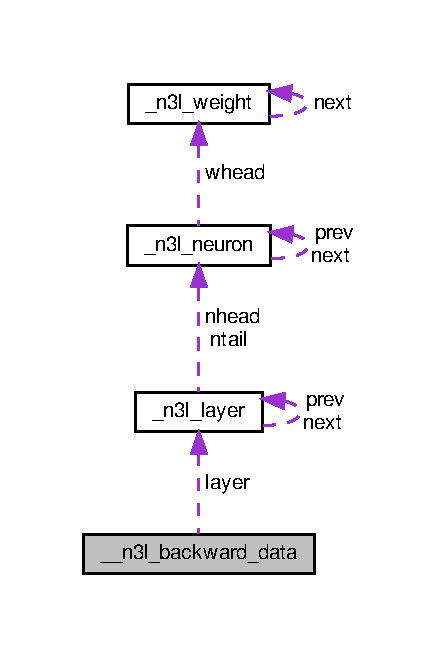
\includegraphics[width=210pt]{struct____n3l__backward__data__coll__graph}
\end{center}
\end{figure}
\subsection*{Data Fields}
\begin{DoxyCompactItemize}
\item 
uint64\+\_\+t \hyperlink{struct____n3l__backward__data_a32ef8a9b7e79121a563b8cd5486f88d3}{ref}
\item 
\hyperlink{n3__header_8h_a9ee3a7104816bdb6222148cfe9ca8ad9}{N3\+L\+Layer} $\ast$ \hyperlink{struct____n3l__backward__data_a0dcc17f32256df3e7ec65046236ffd24}{layer}
\item 
double \hyperlink{struct____n3l__backward__data_ab41bb2c143496d239fe41b208809cc85}{delta}
\item 
double \hyperlink{struct____n3l__backward__data_aa29c1bf7dcb85bfaaa0ec9b01cecc425}{learning\+\_\+rate}
\end{DoxyCompactItemize}


\subsection{Detailed Description}
Internal struct to share data between threads. 

Initialized from the current layer to the previous one. 

\subsection{Field Documentation}
\mbox{\Hypertarget{struct____n3l__backward__data_ab41bb2c143496d239fe41b208809cc85}\label{struct____n3l__backward__data_ab41bb2c143496d239fe41b208809cc85}} 
\index{\+\_\+\+\_\+n3l\+\_\+backward\+\_\+data@{\+\_\+\+\_\+n3l\+\_\+backward\+\_\+data}!delta@{delta}}
\index{delta@{delta}!\+\_\+\+\_\+n3l\+\_\+backward\+\_\+data@{\+\_\+\+\_\+n3l\+\_\+backward\+\_\+data}}
\subsubsection{\texorpdfstring{delta}{delta}}
{\footnotesize\ttfamily double \+\_\+\+\_\+n3l\+\_\+backward\+\_\+data\+::delta}

Delta evaluated \mbox{\Hypertarget{struct____n3l__backward__data_a0dcc17f32256df3e7ec65046236ffd24}\label{struct____n3l__backward__data_a0dcc17f32256df3e7ec65046236ffd24}} 
\index{\+\_\+\+\_\+n3l\+\_\+backward\+\_\+data@{\+\_\+\+\_\+n3l\+\_\+backward\+\_\+data}!layer@{layer}}
\index{layer@{layer}!\+\_\+\+\_\+n3l\+\_\+backward\+\_\+data@{\+\_\+\+\_\+n3l\+\_\+backward\+\_\+data}}
\subsubsection{\texorpdfstring{layer}{layer}}
{\footnotesize\ttfamily \hyperlink{n3__header_8h_a9ee3a7104816bdb6222148cfe9ca8ad9}{N3\+L\+Layer}$\ast$ \+\_\+\+\_\+n3l\+\_\+backward\+\_\+data\+::layer}

Previous layer \mbox{\Hypertarget{struct____n3l__backward__data_aa29c1bf7dcb85bfaaa0ec9b01cecc425}\label{struct____n3l__backward__data_aa29c1bf7dcb85bfaaa0ec9b01cecc425}} 
\index{\+\_\+\+\_\+n3l\+\_\+backward\+\_\+data@{\+\_\+\+\_\+n3l\+\_\+backward\+\_\+data}!learning\+\_\+rate@{learning\+\_\+rate}}
\index{learning\+\_\+rate@{learning\+\_\+rate}!\+\_\+\+\_\+n3l\+\_\+backward\+\_\+data@{\+\_\+\+\_\+n3l\+\_\+backward\+\_\+data}}
\subsubsection{\texorpdfstring{learning\+\_\+rate}{learning\_rate}}
{\footnotesize\ttfamily double \+\_\+\+\_\+n3l\+\_\+backward\+\_\+data\+::learning\+\_\+rate}

Learning rate set to the net \mbox{\Hypertarget{struct____n3l__backward__data_a32ef8a9b7e79121a563b8cd5486f88d3}\label{struct____n3l__backward__data_a32ef8a9b7e79121a563b8cd5486f88d3}} 
\index{\+\_\+\+\_\+n3l\+\_\+backward\+\_\+data@{\+\_\+\+\_\+n3l\+\_\+backward\+\_\+data}!ref@{ref}}
\index{ref@{ref}!\+\_\+\+\_\+n3l\+\_\+backward\+\_\+data@{\+\_\+\+\_\+n3l\+\_\+backward\+\_\+data}}
\subsubsection{\texorpdfstring{ref}{ref}}
{\footnotesize\ttfamily uint64\+\_\+t \+\_\+\+\_\+n3l\+\_\+backward\+\_\+data\+::ref}

Out neuron reference id 

The documentation for this struct was generated from the following file\+:\begin{DoxyCompactItemize}
\item 
src/\hyperlink{n3__backward_8c}{n3\+\_\+backward.\+c}\end{DoxyCompactItemize}

\hypertarget{struct____n3l__forward__data}{}\section{\+\_\+\+\_\+n3l\+\_\+forward\+\_\+data Struct Reference}
\label{struct____n3l__forward__data}\index{\+\_\+\+\_\+n3l\+\_\+forward\+\_\+data@{\+\_\+\+\_\+n3l\+\_\+forward\+\_\+data}}


Internal struct to share data between threads.  




Collaboration diagram for \+\_\+\+\_\+n3l\+\_\+forward\+\_\+data\+:
\nopagebreak
\begin{figure}[H]
\begin{center}
\leavevmode
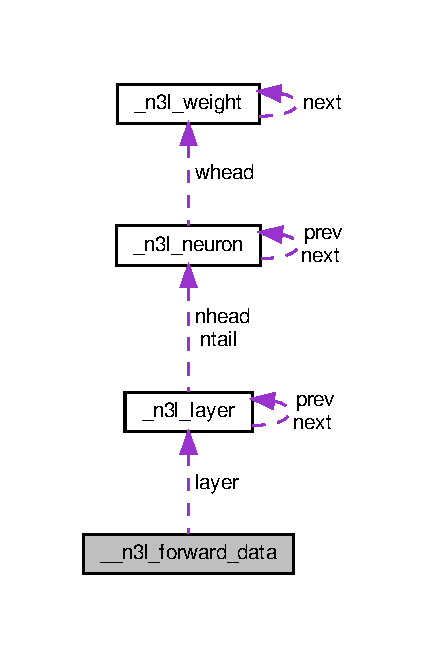
\includegraphics[width=205pt]{struct____n3l__forward__data__coll__graph}
\end{center}
\end{figure}
\subsection*{Data Fields}
\begin{DoxyCompactItemize}
\item 
uint64\+\_\+t \hyperlink{struct____n3l__forward__data_ada78b9bd1418f8dccab76319afb7d64b}{ref}
\item 
\hyperlink{n3__header_8h_a9ee3a7104816bdb6222148cfe9ca8ad9}{N3\+L\+Layer} $\ast$ \hyperlink{struct____n3l__forward__data_aaeb45910cc54c7f3a770dbd124477fc2}{layer}
\item 
double $\ast$ \hyperlink{struct____n3l__forward__data_ac870eae5ce14b297b5d78cc7112c8cec}{result}
\end{DoxyCompactItemize}


\subsection{Detailed Description}
Internal struct to share data between threads. 

Initialized from the current layer to the next one.

\begin{DoxySeeAlso}{See also}
\hyperlink{n3__forward_8c_ac55d957c2a3b754387f5037e87317870}{\+\_\+\+\_\+n3l\+\_\+forward\+\_\+get\+\_\+outputs} 
\end{DoxySeeAlso}


\subsection{Field Documentation}
\mbox{\Hypertarget{struct____n3l__forward__data_aaeb45910cc54c7f3a770dbd124477fc2}\label{struct____n3l__forward__data_aaeb45910cc54c7f3a770dbd124477fc2}} 
\index{\+\_\+\+\_\+n3l\+\_\+forward\+\_\+data@{\+\_\+\+\_\+n3l\+\_\+forward\+\_\+data}!layer@{layer}}
\index{layer@{layer}!\+\_\+\+\_\+n3l\+\_\+forward\+\_\+data@{\+\_\+\+\_\+n3l\+\_\+forward\+\_\+data}}
\subsubsection{\texorpdfstring{layer}{layer}}
{\footnotesize\ttfamily \hyperlink{n3__header_8h_a9ee3a7104816bdb6222148cfe9ca8ad9}{N3\+L\+Layer}$\ast$ \+\_\+\+\_\+n3l\+\_\+forward\+\_\+data\+::layer}

Current layer \mbox{\Hypertarget{struct____n3l__forward__data_ada78b9bd1418f8dccab76319afb7d64b}\label{struct____n3l__forward__data_ada78b9bd1418f8dccab76319afb7d64b}} 
\index{\+\_\+\+\_\+n3l\+\_\+forward\+\_\+data@{\+\_\+\+\_\+n3l\+\_\+forward\+\_\+data}!ref@{ref}}
\index{ref@{ref}!\+\_\+\+\_\+n3l\+\_\+forward\+\_\+data@{\+\_\+\+\_\+n3l\+\_\+forward\+\_\+data}}
\subsubsection{\texorpdfstring{ref}{ref}}
{\footnotesize\ttfamily uint64\+\_\+t \+\_\+\+\_\+n3l\+\_\+forward\+\_\+data\+::ref}

Next layer\textquotesingle{}s neuron reference \mbox{\Hypertarget{struct____n3l__forward__data_ac870eae5ce14b297b5d78cc7112c8cec}\label{struct____n3l__forward__data_ac870eae5ce14b297b5d78cc7112c8cec}} 
\index{\+\_\+\+\_\+n3l\+\_\+forward\+\_\+data@{\+\_\+\+\_\+n3l\+\_\+forward\+\_\+data}!result@{result}}
\index{result@{result}!\+\_\+\+\_\+n3l\+\_\+forward\+\_\+data@{\+\_\+\+\_\+n3l\+\_\+forward\+\_\+data}}
\subsubsection{\texorpdfstring{result}{result}}
{\footnotesize\ttfamily double$\ast$ \+\_\+\+\_\+n3l\+\_\+forward\+\_\+data\+::result}

Sum result while collecting outputs function 

The documentation for this struct was generated from the following file\+:\begin{DoxyCompactItemize}
\item 
src/\hyperlink{n3__forward_8c}{n3\+\_\+forward.\+c}\end{DoxyCompactItemize}

\hypertarget{struct__n3l__layer}{}\section{\+\_\+n3l\+\_\+layer Struct Reference}
\label{struct__n3l__layer}\index{\+\_\+n3l\+\_\+layer@{\+\_\+n3l\+\_\+layer}}


Double Linked List which contains layer\textquotesingle{}s values.  




{\ttfamily \#include $<$n3\+\_\+header.\+h$>$}



Collaboration diagram for \+\_\+n3l\+\_\+layer\+:\nopagebreak
\begin{figure}[H]
\begin{center}
\leavevmode
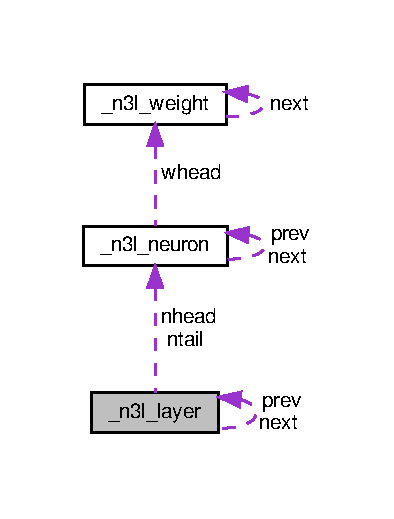
\includegraphics[width=189pt]{struct__n3l__layer__coll__graph}
\end{center}
\end{figure}
\subsection*{Data Fields}
\begin{DoxyCompactItemize}
\item 
\hyperlink{n3__header_8h_a1040baea07fec4d26d25641f75e892c5}{N3\+L\+Layer\+Type} \hyperlink{struct__n3l__layer_aec180f7f12ea86bb622c364076dbf1f6}{type}
\item 
\hyperlink{n3__header_8h_a621b1df037f351bd3542298933e5799a}{N3\+L\+Neuron} $\ast$ \hyperlink{struct__n3l__layer_a263e7831428a3b535964412a1d802c4e}{nhead}
\item 
\hyperlink{n3__header_8h_a621b1df037f351bd3542298933e5799a}{N3\+L\+Neuron} $\ast$ \hyperlink{struct__n3l__layer_aa120fe4ab0898e733b8d6940b467ebc3}{ntail}
\item 
struct \hyperlink{struct__n3l__layer}{\+\_\+n3l\+\_\+layer} $\ast$ \hyperlink{struct__n3l__layer_afada0fe8b2a403d5aeeb71b0ae7f8aae}{next}
\item 
struct \hyperlink{struct__n3l__layer}{\+\_\+n3l\+\_\+layer} $\ast$ \hyperlink{struct__n3l__layer_aedfd507c2c60e3b64234b8cd8570e6c9}{prev}
\end{DoxyCompactItemize}


\subsection{Detailed Description}
Double Linked List which contains layer\textquotesingle{}s values. 

The list is built by \hyperlink{n3__network_8c_a5f87e1efebd658dd55d7d2ca1768bdba}{n3l\+\_\+network\+\_\+build()} or \hyperlink{n3__file_8c_a4fef76548ed87845dceafaa9527a83d0}{n3l\+\_\+file\+\_\+import\+\_\+network()}.

\begin{DoxySeeAlso}{See also}
\hyperlink{struct__n3l__neuron}{\+\_\+n3l\+\_\+neuron}, \hyperlink{structN3LNetwork}{N3\+L\+Network}, \hyperlink{n3__layer_8c_a135215adb7cf8420293fd4ebd7049655}{n3l\+\_\+layer\+\_\+build}, \hyperlink{n3__layer_8c_ab06afb58d55be21a00bde5ee840f6425}{n3l\+\_\+layer\+\_\+count}, \hyperlink{n3__layer_8c_ad58e1630c1b7fc5da03d54cf63c394d9}{n3l\+\_\+layer\+\_\+free} 
\end{DoxySeeAlso}


\subsection{Field Documentation}
\mbox{\Hypertarget{struct__n3l__layer_afada0fe8b2a403d5aeeb71b0ae7f8aae}\label{struct__n3l__layer_afada0fe8b2a403d5aeeb71b0ae7f8aae}} 
\index{\+\_\+n3l\+\_\+layer@{\+\_\+n3l\+\_\+layer}!next@{next}}
\index{next@{next}!\+\_\+n3l\+\_\+layer@{\+\_\+n3l\+\_\+layer}}
\subsubsection{\texorpdfstring{next}{next}}
{\footnotesize\ttfamily struct \hyperlink{struct__n3l__layer}{\+\_\+n3l\+\_\+layer}$\ast$ \+\_\+n3l\+\_\+layer\+::next}

Next layer in the list or N\+U\+LL if it\textquotesingle{}s the last one. \mbox{\Hypertarget{struct__n3l__layer_a263e7831428a3b535964412a1d802c4e}\label{struct__n3l__layer_a263e7831428a3b535964412a1d802c4e}} 
\index{\+\_\+n3l\+\_\+layer@{\+\_\+n3l\+\_\+layer}!nhead@{nhead}}
\index{nhead@{nhead}!\+\_\+n3l\+\_\+layer@{\+\_\+n3l\+\_\+layer}}
\subsubsection{\texorpdfstring{nhead}{nhead}}
{\footnotesize\ttfamily \hyperlink{n3__header_8h_a621b1df037f351bd3542298933e5799a}{N3\+L\+Neuron}$\ast$ \+\_\+n3l\+\_\+layer\+::nhead}

Layer\textquotesingle{}s neuron list head. \begin{DoxySeeAlso}{See also}
\hyperlink{struct__n3l__neuron}{\+\_\+n3l\+\_\+neuron} 
\end{DoxySeeAlso}
\mbox{\Hypertarget{struct__n3l__layer_aa120fe4ab0898e733b8d6940b467ebc3}\label{struct__n3l__layer_aa120fe4ab0898e733b8d6940b467ebc3}} 
\index{\+\_\+n3l\+\_\+layer@{\+\_\+n3l\+\_\+layer}!ntail@{ntail}}
\index{ntail@{ntail}!\+\_\+n3l\+\_\+layer@{\+\_\+n3l\+\_\+layer}}
\subsubsection{\texorpdfstring{ntail}{ntail}}
{\footnotesize\ttfamily \hyperlink{n3__header_8h_a621b1df037f351bd3542298933e5799a}{N3\+L\+Neuron}$\ast$ \+\_\+n3l\+\_\+layer\+::ntail}

Layer\textquotesingle{}s neuron list tail. \begin{DoxySeeAlso}{See also}
\hyperlink{struct__n3l__neuron}{\+\_\+n3l\+\_\+neuron} 
\end{DoxySeeAlso}
\mbox{\Hypertarget{struct__n3l__layer_aedfd507c2c60e3b64234b8cd8570e6c9}\label{struct__n3l__layer_aedfd507c2c60e3b64234b8cd8570e6c9}} 
\index{\+\_\+n3l\+\_\+layer@{\+\_\+n3l\+\_\+layer}!prev@{prev}}
\index{prev@{prev}!\+\_\+n3l\+\_\+layer@{\+\_\+n3l\+\_\+layer}}
\subsubsection{\texorpdfstring{prev}{prev}}
{\footnotesize\ttfamily struct \hyperlink{struct__n3l__layer}{\+\_\+n3l\+\_\+layer}$\ast$ \+\_\+n3l\+\_\+layer\+::prev}

Previous layer in the list or N\+U\+LL if it\textquotesingle{}s the first one. \mbox{\Hypertarget{struct__n3l__layer_aec180f7f12ea86bb622c364076dbf1f6}\label{struct__n3l__layer_aec180f7f12ea86bb622c364076dbf1f6}} 
\index{\+\_\+n3l\+\_\+layer@{\+\_\+n3l\+\_\+layer}!type@{type}}
\index{type@{type}!\+\_\+n3l\+\_\+layer@{\+\_\+n3l\+\_\+layer}}
\subsubsection{\texorpdfstring{type}{type}}
{\footnotesize\ttfamily \hyperlink{n3__header_8h_a1040baea07fec4d26d25641f75e892c5}{N3\+L\+Layer\+Type} \+\_\+n3l\+\_\+layer\+::type}

Layer type. \begin{DoxySeeAlso}{See also}
\hyperlink{n3__header_8h_a1040baea07fec4d26d25641f75e892c5}{N3\+L\+Layer\+Type} 
\end{DoxySeeAlso}


The documentation for this struct was generated from the following file\+:\begin{DoxyCompactItemize}
\item 
src/\hyperlink{n3__header_8h}{n3\+\_\+header.\+h}\end{DoxyCompactItemize}

\hypertarget{struct__n3l__neuron}{}\section{\+\_\+n3l\+\_\+neuron Struct Reference}
\label{struct__n3l__neuron}\index{\+\_\+n3l\+\_\+neuron@{\+\_\+n3l\+\_\+neuron}}


Double Linked List which contains neuron\textquotesingle{}s values.  




{\ttfamily \#include $<$n3\+\_\+header.\+h$>$}



Collaboration diagram for \+\_\+n3l\+\_\+neuron\+:\nopagebreak
\begin{figure}[H]
\begin{center}
\leavevmode
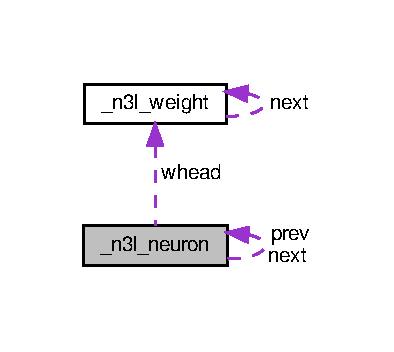
\includegraphics[width=189pt]{struct__n3l__neuron__coll__graph}
\end{center}
\end{figure}
\subsection*{Data Fields}
\begin{DoxyCompactItemize}
\item 
bool \hyperlink{struct__n3l__neuron_a0f3291ff81ab13111e538622ab662069}{bias}
\item 
uint64\+\_\+t \hyperlink{struct__n3l__neuron_aa0053e003b954df3b58853f003284958}{ref}
\item 
double \hyperlink{struct__n3l__neuron_ac896f5f8bd82c056cc61872120391048}{input}
\item 
\hyperlink{n3__header_8h_ac37c67a24ec253f5cd205cbc981922ca}{N3\+L\+Weight} $\ast$ \hyperlink{struct__n3l__neuron_ac9259a513822ea957c03430988adfa6a}{whead}
\item 
double \hyperlink{struct__n3l__neuron_afc9c38f4676dbe2ead749f8b6c81f491}{result}
\item 
\hyperlink{n3__header_8h_a3118e8995213ca26bd388c3d94cd8056}{N3\+L\+Act\+Type} \hyperlink{struct__n3l__neuron_af424e7accb8d1d089b828a1de69e03a0}{act\+\_\+type}
\item 
\hyperlink{n3__header_8h_afb10e6f7012513b51225a4d3add36cae}{N3\+L\+Act} \hyperlink{struct__n3l__neuron_a3ed17ddbe86d42ed6b7d31256b109262}{act}
\item 
\hyperlink{n3__header_8h_afb10e6f7012513b51225a4d3add36cae}{N3\+L\+Act} \hyperlink{struct__n3l__neuron_a9c9de65191cb097fd7a71752c83fc3db}{act\+\_\+prime}
\item 
struct \hyperlink{struct__n3l__neuron}{\+\_\+n3l\+\_\+neuron} $\ast$ \hyperlink{struct__n3l__neuron_a55f1bc3d589d69c5a940d0cb497610c4}{next}
\item 
struct \hyperlink{struct__n3l__neuron}{\+\_\+n3l\+\_\+neuron} $\ast$ \hyperlink{struct__n3l__neuron_a706ad4614fd4d1bd9a824f6ea8c0c9e5}{prev}
\end{DoxyCompactItemize}


\subsection{Detailed Description}
Double Linked List which contains neuron\textquotesingle{}s values. 

The list is built by n3l\+\_\+network\+\_\+build() or \hyperlink{n3__file_8c_a4fef76548ed87845dceafaa9527a83d0}{n3l\+\_\+file\+\_\+import\+\_\+network()}.

\begin{DoxySeeAlso}{See also}
\hyperlink{struct__n3l__layer}{\+\_\+n3l\+\_\+layer}, \hyperlink{struct__n3l__weight}{\+\_\+n3l\+\_\+weight}, n3l\+\_\+neuron\+\_\+build, n3l\+\_\+neuron\+\_\+count, n3l\+\_\+neuron\+\_\+free 
\end{DoxySeeAlso}


\subsection{Field Documentation}
\mbox{\Hypertarget{struct__n3l__neuron_a3ed17ddbe86d42ed6b7d31256b109262}\label{struct__n3l__neuron_a3ed17ddbe86d42ed6b7d31256b109262}} 
\index{\+\_\+n3l\+\_\+neuron@{\+\_\+n3l\+\_\+neuron}!act@{act}}
\index{act@{act}!\+\_\+n3l\+\_\+neuron@{\+\_\+n3l\+\_\+neuron}}
\subsubsection{\texorpdfstring{act}{act}}
{\footnotesize\ttfamily \hyperlink{n3__header_8h_afb10e6f7012513b51225a4d3add36cae}{N3\+L\+Act} \+\_\+n3l\+\_\+neuron\+::act}

Activation function. \begin{DoxySeeAlso}{See also}
\hyperlink{n3__header_8h_afb10e6f7012513b51225a4d3add36cae}{N3\+L\+Act} 
\end{DoxySeeAlso}
\mbox{\Hypertarget{struct__n3l__neuron_a9c9de65191cb097fd7a71752c83fc3db}\label{struct__n3l__neuron_a9c9de65191cb097fd7a71752c83fc3db}} 
\index{\+\_\+n3l\+\_\+neuron@{\+\_\+n3l\+\_\+neuron}!act\+\_\+prime@{act\+\_\+prime}}
\index{act\+\_\+prime@{act\+\_\+prime}!\+\_\+n3l\+\_\+neuron@{\+\_\+n3l\+\_\+neuron}}
\subsubsection{\texorpdfstring{act\+\_\+prime}{act\_prime}}
{\footnotesize\ttfamily \hyperlink{n3__header_8h_afb10e6f7012513b51225a4d3add36cae}{N3\+L\+Act} \+\_\+n3l\+\_\+neuron\+::act\+\_\+prime}

Activation function primitive. \begin{DoxySeeAlso}{See also}
\hyperlink{n3__header_8h_afb10e6f7012513b51225a4d3add36cae}{N3\+L\+Act} 
\end{DoxySeeAlso}
\mbox{\Hypertarget{struct__n3l__neuron_af424e7accb8d1d089b828a1de69e03a0}\label{struct__n3l__neuron_af424e7accb8d1d089b828a1de69e03a0}} 
\index{\+\_\+n3l\+\_\+neuron@{\+\_\+n3l\+\_\+neuron}!act\+\_\+type@{act\+\_\+type}}
\index{act\+\_\+type@{act\+\_\+type}!\+\_\+n3l\+\_\+neuron@{\+\_\+n3l\+\_\+neuron}}
\subsubsection{\texorpdfstring{act\+\_\+type}{act\_type}}
{\footnotesize\ttfamily \hyperlink{n3__header_8h_a3118e8995213ca26bd388c3d94cd8056}{N3\+L\+Act\+Type} \+\_\+n3l\+\_\+neuron\+::act\+\_\+type}

Activation function type. \begin{DoxySeeAlso}{See also}
\hyperlink{n3__header_8h_a3118e8995213ca26bd388c3d94cd8056}{N3\+L\+Act\+Type} 
\end{DoxySeeAlso}
\mbox{\Hypertarget{struct__n3l__neuron_a0f3291ff81ab13111e538622ab662069}\label{struct__n3l__neuron_a0f3291ff81ab13111e538622ab662069}} 
\index{\+\_\+n3l\+\_\+neuron@{\+\_\+n3l\+\_\+neuron}!bias@{bias}}
\index{bias@{bias}!\+\_\+n3l\+\_\+neuron@{\+\_\+n3l\+\_\+neuron}}
\subsubsection{\texorpdfstring{bias}{bias}}
{\footnotesize\ttfamily bool \+\_\+n3l\+\_\+neuron\+::bias}

Identifies if the neuron is a bias neuron. The bias neurons doesn\textquotesingle{}t get inputs and have N3\+L\+None as activation function. \begin{DoxyNote}{Note}
Usually there is only one bias neuron for each layer, except for the output one, and it\textquotesingle{}s built as last neuron.
\end{DoxyNote}
\begin{DoxySeeAlso}{See also}
\hyperlink{n3__act_8c_a8dc073371b15e2574897762b54f9326c}{n3l\+\_\+act\+\_\+none}, \hyperlink{structN3LArgs}{N3\+L\+Args}, n3l\+\_\+network\+\_\+build 
\end{DoxySeeAlso}
\mbox{\Hypertarget{struct__n3l__neuron_ac896f5f8bd82c056cc61872120391048}\label{struct__n3l__neuron_ac896f5f8bd82c056cc61872120391048}} 
\index{\+\_\+n3l\+\_\+neuron@{\+\_\+n3l\+\_\+neuron}!input@{input}}
\index{input@{input}!\+\_\+n3l\+\_\+neuron@{\+\_\+n3l\+\_\+neuron}}
\subsubsection{\texorpdfstring{input}{input}}
{\footnotesize\ttfamily double \+\_\+n3l\+\_\+neuron\+::input}

Neuron input value. This value is also used to apply activation fuction.

\begin{DoxySeeAlso}{See also}
\hyperlink{n3__forward_8c_a658e97e1260b05ef3d286fbe93f11a40}{\+\_\+\+\_\+n3l\+\_\+forward\+\_\+layer} 
\end{DoxySeeAlso}
\mbox{\Hypertarget{struct__n3l__neuron_a55f1bc3d589d69c5a940d0cb497610c4}\label{struct__n3l__neuron_a55f1bc3d589d69c5a940d0cb497610c4}} 
\index{\+\_\+n3l\+\_\+neuron@{\+\_\+n3l\+\_\+neuron}!next@{next}}
\index{next@{next}!\+\_\+n3l\+\_\+neuron@{\+\_\+n3l\+\_\+neuron}}
\subsubsection{\texorpdfstring{next}{next}}
{\footnotesize\ttfamily struct \hyperlink{struct__n3l__neuron}{\+\_\+n3l\+\_\+neuron}$\ast$ \+\_\+n3l\+\_\+neuron\+::next}

Next neuron in the list or N\+U\+LL if it\textquotesingle{}s the last one. \mbox{\Hypertarget{struct__n3l__neuron_a706ad4614fd4d1bd9a824f6ea8c0c9e5}\label{struct__n3l__neuron_a706ad4614fd4d1bd9a824f6ea8c0c9e5}} 
\index{\+\_\+n3l\+\_\+neuron@{\+\_\+n3l\+\_\+neuron}!prev@{prev}}
\index{prev@{prev}!\+\_\+n3l\+\_\+neuron@{\+\_\+n3l\+\_\+neuron}}
\subsubsection{\texorpdfstring{prev}{prev}}
{\footnotesize\ttfamily struct \hyperlink{struct__n3l__neuron}{\+\_\+n3l\+\_\+neuron}$\ast$ \+\_\+n3l\+\_\+neuron\+::prev}

Previous neuron in the list or N\+U\+LL if it\textquotesingle{}s the first one. \mbox{\Hypertarget{struct__n3l__neuron_aa0053e003b954df3b58853f003284958}\label{struct__n3l__neuron_aa0053e003b954df3b58853f003284958}} 
\index{\+\_\+n3l\+\_\+neuron@{\+\_\+n3l\+\_\+neuron}!ref@{ref}}
\index{ref@{ref}!\+\_\+n3l\+\_\+neuron@{\+\_\+n3l\+\_\+neuron}}
\subsubsection{\texorpdfstring{ref}{ref}}
{\footnotesize\ttfamily uint64\+\_\+t \+\_\+n3l\+\_\+neuron\+::ref}

Current neuron reference. \begin{DoxyWarning}{Warning}
This value must be unique into the network. It is used to collecting outputs in forward propagation and to evaluate delta in backward propagation.
\end{DoxyWarning}
\begin{DoxySeeAlso}{See also}
\hyperlink{n3__forward_8c_ac55d957c2a3b754387f5037e87317870}{\+\_\+\+\_\+n3l\+\_\+forward\+\_\+get\+\_\+outputs}, \hyperlink{n3__backward_8c_accf39951eeeca43985b286831dd397ce}{\+\_\+\+\_\+n3l\+\_\+backward\+\_\+execute} 
\end{DoxySeeAlso}
\mbox{\Hypertarget{struct__n3l__neuron_afc9c38f4676dbe2ead749f8b6c81f491}\label{struct__n3l__neuron_afc9c38f4676dbe2ead749f8b6c81f491}} 
\index{\+\_\+n3l\+\_\+neuron@{\+\_\+n3l\+\_\+neuron}!result@{result}}
\index{result@{result}!\+\_\+n3l\+\_\+neuron@{\+\_\+n3l\+\_\+neuron}}
\subsubsection{\texorpdfstring{result}{result}}
{\footnotesize\ttfamily double \+\_\+n3l\+\_\+neuron\+::result}

Neuron\textquotesingle{}s result. This value is initialiazed after forward propagation.

\begin{DoxySeeAlso}{See also}
\hyperlink{n3__forward_8c_abc37ac7f137db4d053e3b19ac8e6542a}{n3l\+\_\+forward\+\_\+propagation}, \hyperlink{n3__forward_8c_af014464aaf6842d7da0ee6d1b1570ffe}{\+\_\+\+\_\+n3l\+\_\+forward\+\_\+activate} 
\end{DoxySeeAlso}
\mbox{\Hypertarget{struct__n3l__neuron_ac9259a513822ea957c03430988adfa6a}\label{struct__n3l__neuron_ac9259a513822ea957c03430988adfa6a}} 
\index{\+\_\+n3l\+\_\+neuron@{\+\_\+n3l\+\_\+neuron}!whead@{whead}}
\index{whead@{whead}!\+\_\+n3l\+\_\+neuron@{\+\_\+n3l\+\_\+neuron}}
\subsubsection{\texorpdfstring{whead}{whead}}
{\footnotesize\ttfamily \hyperlink{n3__header_8h_ac37c67a24ec253f5cd205cbc981922ca}{N3\+L\+Weight}$\ast$ \+\_\+n3l\+\_\+neuron\+::whead}

Weight\textquotesingle{}s list head. \begin{DoxyNote}{Note}
It is set to N\+U\+LL if the neuron\textquotesingle{}s layer is of type N3\+L\+Output\+Layer
\end{DoxyNote}
\begin{DoxySeeAlso}{See also}
\hyperlink{struct__n3l__weight}{\+\_\+n3l\+\_\+weight}, \hyperlink{struct__n3l__layer}{\+\_\+n3l\+\_\+layer} 
\end{DoxySeeAlso}


The documentation for this struct was generated from the following file\+:\begin{DoxyCompactItemize}
\item 
src/\hyperlink{n3__header_8h}{n3\+\_\+header.\+h}\end{DoxyCompactItemize}

\hypertarget{struct__n3l__weight}{}\section{\+\_\+n3l\+\_\+weight Struct Reference}
\label{struct__n3l__weight}\index{\+\_\+n3l\+\_\+weight@{\+\_\+n3l\+\_\+weight}}


Collaboration diagram for \+\_\+n3l\+\_\+weight\+:\nopagebreak
\begin{figure}[H]
\begin{center}
\leavevmode
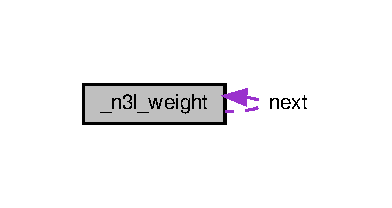
\includegraphics[width=188pt]{struct__n3l__weight__coll__graph}
\end{center}
\end{figure}
\subsection*{Data Fields}
\begin{DoxyCompactItemize}
\item 
\mbox{\Hypertarget{struct__n3l__weight_a1d1ebc5e04ba1dd26094993dd94aa710}\label{struct__n3l__weight_a1d1ebc5e04ba1dd26094993dd94aa710}} 
double {\bfseries value}
\item 
\mbox{\Hypertarget{struct__n3l__weight_ac5094b52f09a092ffb1cdc4cc594f38f}\label{struct__n3l__weight_ac5094b52f09a092ffb1cdc4cc594f38f}} 
uint64\+\_\+t {\bfseries target\+\_\+ref}
\item 
\mbox{\Hypertarget{struct__n3l__weight_adf96faae4820538377678c82ec96d48e}\label{struct__n3l__weight_adf96faae4820538377678c82ec96d48e}} 
struct \hyperlink{struct__n3l__weight}{\+\_\+n3l\+\_\+weight} $\ast$ {\bfseries next}
\end{DoxyCompactItemize}


The documentation for this struct was generated from the following file\+:\begin{DoxyCompactItemize}
\item 
src/n3\+\_\+header.\+h\end{DoxyCompactItemize}

\hypertarget{structN3LArgs}{}\section{N3\+L\+Args Struct Reference}
\label{structN3LArgs}\index{N3\+L\+Args@{N3\+L\+Args}}
\subsection*{Data Fields}
\begin{DoxyCompactItemize}
\item 
\mbox{\Hypertarget{structN3LArgs_ad51d108eba4b55f7fc49174724fbacad}\label{structN3LArgs_ad51d108eba4b55f7fc49174724fbacad}} 
double {\bfseries bias}
\item 
\mbox{\Hypertarget{structN3LArgs_afbd19ab7f7afe11e440f46d293a0f6dc}\label{structN3LArgs_afbd19ab7f7afe11e440f46d293a0f6dc}} 
uint64\+\_\+t {\bfseries in\+\_\+size}
\item 
\mbox{\Hypertarget{structN3LArgs_acbb947695cd6db88658a2a6fa78c1682}\label{structN3LArgs_acbb947695cd6db88658a2a6fa78c1682}} 
uint64\+\_\+t {\bfseries h\+\_\+layers}
\item 
\mbox{\Hypertarget{structN3LArgs_ae875ef755586a29387def48249c98d81}\label{structN3LArgs_ae875ef755586a29387def48249c98d81}} 
uint64\+\_\+t $\ast$ {\bfseries h\+\_\+size}
\item 
\mbox{\Hypertarget{structN3LArgs_a63bb20896b0af109ea281998e5fd56ab}\label{structN3LArgs_a63bb20896b0af109ea281998e5fd56ab}} 
uint64\+\_\+t {\bfseries out\+\_\+size}
\item 
\mbox{\Hypertarget{structN3LArgs_abb810a671b7a1b20c161e81e309f843c}\label{structN3LArgs_abb810a671b7a1b20c161e81e309f843c}} 
N3\+L\+Act\+Type {\bfseries act\+\_\+in}
\item 
\mbox{\Hypertarget{structN3LArgs_a968aa1ed194fc7bbfaac154bcbf8a405}\label{structN3LArgs_a968aa1ed194fc7bbfaac154bcbf8a405}} 
N3\+L\+Act\+Type $\ast$ {\bfseries act\+\_\+h}
\item 
\mbox{\Hypertarget{structN3LArgs_ad9d17026b32668acea535143809b16c5}\label{structN3LArgs_ad9d17026b32668acea535143809b16c5}} 
N3\+L\+Act\+Type {\bfseries act\+\_\+out}
\item 
\mbox{\Hypertarget{structN3LArgs_a9df79247b5160e5261683a535654cc18}\label{structN3LArgs_a9df79247b5160e5261683a535654cc18}} 
void $\ast$ {\bfseries rand\+\_\+arg}
\item 
\mbox{\Hypertarget{structN3LArgs_ac6f4a8939deb104e8b154860904f3b45}\label{structN3LArgs_ac6f4a8939deb104e8b154860904f3b45}} 
N3\+L\+Weight\+Generator {\bfseries rand\+\_\+weight}
\end{DoxyCompactItemize}


The documentation for this struct was generated from the following file\+:\begin{DoxyCompactItemize}
\item 
src/n3\+\_\+header.\+h\end{DoxyCompactItemize}

\hypertarget{structN3LNetwork}{}\section{N3\+L\+Network Struct Reference}
\label{structN3LNetwork}\index{N3\+L\+Network@{N3\+L\+Network}}


Collaboration diagram for N3\+L\+Network\+:\nopagebreak
\begin{figure}[H]
\begin{center}
\leavevmode
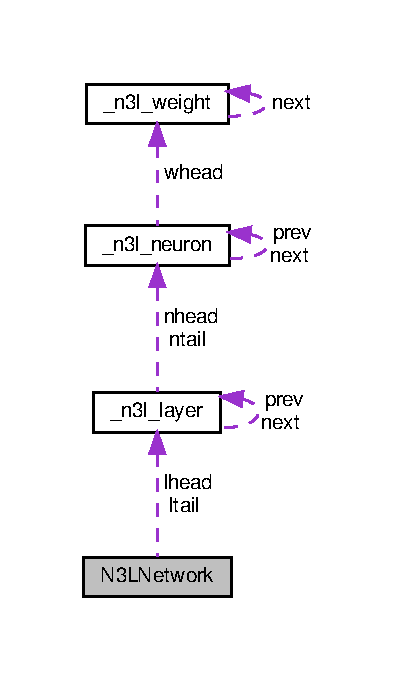
\includegraphics[width=190pt]{structN3LNetwork__coll__graph}
\end{center}
\end{figure}
\subsection*{Data Fields}
\begin{DoxyCompactItemize}
\item 
\mbox{\Hypertarget{structN3LNetwork_a45ff5bcae18502559925aba0cbd0313b}\label{structN3LNetwork_a45ff5bcae18502559925aba0cbd0313b}} 
double $\ast$ {\bfseries inputs}
\item 
\mbox{\Hypertarget{structN3LNetwork_aba0f6767a66173743840b7c9fa919daf}\label{structN3LNetwork_aba0f6767a66173743840b7c9fa919daf}} 
double $\ast$ {\bfseries targets}
\item 
\mbox{\Hypertarget{structN3LNetwork_ae7c5e2ed74786685185cf2cbb955bf51}\label{structN3LNetwork_ae7c5e2ed74786685185cf2cbb955bf51}} 
double {\bfseries learning\+\_\+rate}
\item 
\mbox{\Hypertarget{structN3LNetwork_ae77d4b7deecdc3c9590a4112689db2f8}\label{structN3LNetwork_ae77d4b7deecdc3c9590a4112689db2f8}} 
\hyperlink{struct__n3l__layer}{N3\+L\+Layer} $\ast$ {\bfseries lhead}
\item 
\mbox{\Hypertarget{structN3LNetwork_a758fd06b3dda29e064ccd4bc4d27e1c3}\label{structN3LNetwork_a758fd06b3dda29e064ccd4bc4d27e1c3}} 
\hyperlink{struct__n3l__layer}{N3\+L\+Layer} $\ast$ {\bfseries ltail}
\end{DoxyCompactItemize}


The documentation for this struct was generated from the following file\+:\begin{DoxyCompactItemize}
\item 
src/n3\+\_\+header.\+h\end{DoxyCompactItemize}

\chapter{File Documentation}
\hypertarget{n3__act_8c}{}\section{src/n3\+\_\+act.c File Reference}
\label{n3__act_8c}\index{src/n3\+\_\+act.\+c@{src/n3\+\_\+act.\+c}}


This file contains activation functions and their primitive.  


{\ttfamily \#include $<$assert.\+h$>$}\newline
{\ttfamily \#include $<$math.\+h$>$}\newline
{\ttfamily \#include \char`\"{}n3\+\_\+header.\+h\char`\"{}}\newline
Include dependency graph for n3\+\_\+act.\+c\+:\nopagebreak
\begin{figure}[H]
\begin{center}
\leavevmode
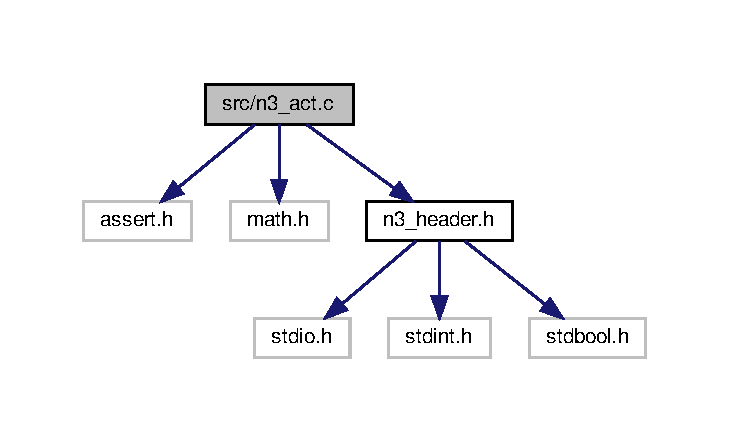
\includegraphics[width=350pt]{n3__act_8c__incl}
\end{center}
\end{figure}
\subsection*{Macros}
\begin{DoxyCompactItemize}
\item 
\#define \mbox{\hyperlink{n3__act_8c_a5347f97ed167ced1e9ffb374f218d479}{N3\+L\+\_\+\+A\+BS}}(x)~(((x) $<$ 0) ? -\/(x) \+: (x))
\begin{DoxyCompactList}\small\item\em Get the absolute value of the argument passed. \end{DoxyCompactList}\end{DoxyCompactItemize}
\subsection*{Functions}
\begin{DoxyCompactItemize}
\item 
double \mbox{\hyperlink{n3__act_8c_a8dc073371b15e2574897762b54f9326c}{n3l\+\_\+act\+\_\+none}} (double val)
\begin{DoxyCompactList}\small\item\em Doesn\textquotesingle{}t change the value passed as argument. \end{DoxyCompactList}\item 
double \mbox{\hyperlink{n3__act_8c_ad01dde283500e1fbac8d916967bfd883}{n3l\+\_\+act\+\_\+sigmoid}} (double val)
\begin{DoxyCompactList}\small\item\em Sigmoid activation function. \end{DoxyCompactList}\item 
double \mbox{\hyperlink{n3__act_8c_a4c1864b101c16c51e69a34b130fc30b6}{n3l\+\_\+act\+\_\+sigmoid\+\_\+prime}} (double val)
\begin{DoxyCompactList}\small\item\em Sigmoid activation primitive function. \end{DoxyCompactList}\item 
double \mbox{\hyperlink{n3__act_8c_aa05576ce02d1c18c0af9f042d1068c7a}{n3l\+\_\+act\+\_\+tanh}} (double val)
\begin{DoxyCompactList}\small\item\em Tanh activation function. \end{DoxyCompactList}\item 
double \mbox{\hyperlink{n3__act_8c_a24f63de53f6417037d5bebec78e08870}{n3l\+\_\+act\+\_\+tanh\+\_\+prime}} (double val)
\begin{DoxyCompactList}\small\item\em Tanh activation primitive function. \end{DoxyCompactList}\item 
double \mbox{\hyperlink{n3__act_8c_a07a8cded25f1d3b726053b50cba78eb0}{n3l\+\_\+act\+\_\+relu}} (double val)
\begin{DoxyCompactList}\small\item\em Re\+LU activation function. \end{DoxyCompactList}\item 
double \mbox{\hyperlink{n3__act_8c_ae94558725d2c300ef0879b83ee5e733a}{n3l\+\_\+act\+\_\+relu\+\_\+prime}} (double val)
\begin{DoxyCompactList}\small\item\em Re\+LU activation primitive function. \end{DoxyCompactList}\item 
double \mbox{\hyperlink{n3__act_8c_a066f6fed961da89043b1b496aa5ac6d0}{n3l\+\_\+act\+\_\+identity}} (double val)
\begin{DoxyCompactList}\small\item\em Identity activation function. \end{DoxyCompactList}\item 
double \mbox{\hyperlink{n3__act_8c_a7706b52da3c207ee1ded39ced860a138}{n3l\+\_\+act\+\_\+identity\+\_\+prime}} (double val)
\begin{DoxyCompactList}\small\item\em Identity activation primitive function. \end{DoxyCompactList}\item 
double \mbox{\hyperlink{n3__act_8c_a9e9cd6045617a4063602ccd9e94281bf}{n3l\+\_\+act\+\_\+softsign}} (double val)
\begin{DoxyCompactList}\small\item\em Soft\+Sign activation function. \end{DoxyCompactList}\item 
double \mbox{\hyperlink{n3__act_8c_aeb7c71c9bb444a3a875b7838064c8bb4}{n3l\+\_\+act\+\_\+softsign\+\_\+prime}} (double val)
\begin{DoxyCompactList}\small\item\em Soft\+Sign activation primitive function. \end{DoxyCompactList}\item 
double \mbox{\hyperlink{n3__act_8c_a2091491a8d0155701b6170c324b52eef}{n3l\+\_\+act\+\_\+leaky\+\_\+relu}} (double val)
\begin{DoxyCompactList}\small\item\em Leaky Re\+LU activation function. \end{DoxyCompactList}\item 
double \mbox{\hyperlink{n3__act_8c_a326894c0edd659426f5deaec6abe5182}{n3l\+\_\+act\+\_\+leaky\+\_\+relu\+\_\+prime}} (double val)
\begin{DoxyCompactList}\small\item\em Leaky Re\+LU activation primitive function. \end{DoxyCompactList}\item 
double \mbox{\hyperlink{n3__act_8c_ab678727eab04c73e227d0511f10da9ab}{n3l\+\_\+act\+\_\+softplus}} (double val)
\begin{DoxyCompactList}\small\item\em Soft\+Plus activation function. \end{DoxyCompactList}\item 
double \mbox{\hyperlink{n3__act_8c_a405fc712bf5abf365c90a343c664c273}{n3l\+\_\+act\+\_\+softplus\+\_\+prime}} (double val)
\begin{DoxyCompactList}\small\item\em Soft\+Plus activation primitive function. \end{DoxyCompactList}\item 
double \mbox{\hyperlink{n3__act_8c_a64fdb17c0915027691ad0b1340bdb1af}{n3l\+\_\+act\+\_\+swish}} (double val)
\begin{DoxyCompactList}\small\item\em Swish activation function. \end{DoxyCompactList}\item 
double \mbox{\hyperlink{n3__act_8c_ac0171e96a4e3c4220a4a0353e77f042b}{n3l\+\_\+act\+\_\+swish\+\_\+prime}} (double val)
\begin{DoxyCompactList}\small\item\em Swish activation primitive function. \end{DoxyCompactList}\item 
N3\+L\+Act \mbox{\hyperlink{n3__act_8c_af9034678bae2b94ebcf0d9b2ac5cfcb7}{n3l\+\_\+act}} (N3\+L\+Act\+Type type)
\begin{DoxyCompactList}\small\item\em Get the pointer to an activation function. \end{DoxyCompactList}\item 
N3\+L\+Act \mbox{\hyperlink{n3__act_8c_a9253520cb5a58edf61f04997c3161f21}{n3l\+\_\+act\+\_\+prime}} (N3\+L\+Act\+Type type)
\begin{DoxyCompactList}\small\item\em Get the pointer to an activation primitive function. \end{DoxyCompactList}\end{DoxyCompactItemize}


\subsection{Detailed Description}
This file contains activation functions and their primitive. 

\begin{DoxyAuthor}{Author}
Davide Francesco Merico 
\end{DoxyAuthor}
\begin{DoxySeeAlso}{See also}
\href{https://en.wikipedia.org/wiki/Activation_function}{\tt Wikipedia -\/ Activation Function} 
\end{DoxySeeAlso}
\begin{DoxyNote}{Note}
These functions, except for n3l\+\_\+act or n3l\+\_\+act\+\_\+prime, shouldn\textquotesingle{}t be used directly to improve compatibility with future library versions. 
\end{DoxyNote}


\subsection{Macro Definition Documentation}
\mbox{\Hypertarget{n3__act_8c_a5347f97ed167ced1e9ffb374f218d479}\label{n3__act_8c_a5347f97ed167ced1e9ffb374f218d479}} 
\index{n3\+\_\+act.\+c@{n3\+\_\+act.\+c}!N3\+L\+\_\+\+A\+BS@{N3\+L\+\_\+\+A\+BS}}
\index{N3\+L\+\_\+\+A\+BS@{N3\+L\+\_\+\+A\+BS}!n3\+\_\+act.\+c@{n3\+\_\+act.\+c}}
\subsubsection{\texorpdfstring{N3\+L\+\_\+\+A\+BS}{N3L\_ABS}}
{\footnotesize\ttfamily \#define N3\+L\+\_\+\+A\+BS(\begin{DoxyParamCaption}\item[{}]{x }\end{DoxyParamCaption})~(((x) $<$ 0) ? -\/(x) \+: (x))}



Get the absolute value of the argument passed. 


\begin{DoxyParams}{Parameters}
{\em x} & value \\
\hline
\end{DoxyParams}
\begin{DoxyReturn}{Returns}
x if x is positive, otherwise -\/x. 
\end{DoxyReturn}


\subsection{Function Documentation}
\mbox{\Hypertarget{n3__act_8c_af9034678bae2b94ebcf0d9b2ac5cfcb7}\label{n3__act_8c_af9034678bae2b94ebcf0d9b2ac5cfcb7}} 
\index{n3\+\_\+act.\+c@{n3\+\_\+act.\+c}!n3l\+\_\+act@{n3l\+\_\+act}}
\index{n3l\+\_\+act@{n3l\+\_\+act}!n3\+\_\+act.\+c@{n3\+\_\+act.\+c}}
\subsubsection{\texorpdfstring{n3l\+\_\+act()}{n3l\_act()}}
{\footnotesize\ttfamily N3\+L\+Act n3l\+\_\+act (\begin{DoxyParamCaption}\item[{N3\+L\+Act\+Type}]{type }\end{DoxyParamCaption})}



Get the pointer to an activation function. 


\begin{DoxyParams}{Parameters}
{\em type} & Activation function type. \\
\hline
\end{DoxyParams}
\begin{DoxyReturn}{Returns}
Pointer to the function chosen.
\end{DoxyReturn}
\begin{DoxySeeAlso}{See also}
\mbox{\hyperlink{n3__act_8c_a9253520cb5a58edf61f04997c3161f21}{n3l\+\_\+act\+\_\+prime}}, N3\+L\+Act, N3\+L\+Act\+Tye 
\end{DoxySeeAlso}
\mbox{\Hypertarget{n3__act_8c_a066f6fed961da89043b1b496aa5ac6d0}\label{n3__act_8c_a066f6fed961da89043b1b496aa5ac6d0}} 
\index{n3\+\_\+act.\+c@{n3\+\_\+act.\+c}!n3l\+\_\+act\+\_\+identity@{n3l\+\_\+act\+\_\+identity}}
\index{n3l\+\_\+act\+\_\+identity@{n3l\+\_\+act\+\_\+identity}!n3\+\_\+act.\+c@{n3\+\_\+act.\+c}}
\subsubsection{\texorpdfstring{n3l\+\_\+act\+\_\+identity()}{n3l\_act\_identity()}}
{\footnotesize\ttfamily double n3l\+\_\+act\+\_\+identity (\begin{DoxyParamCaption}\item[{double}]{val }\end{DoxyParamCaption})}



Identity activation function. 

\[identity(value) = value\]


\begin{DoxyParams}{Parameters}
{\em val} & input value \\
\hline
\end{DoxyParams}
\begin{DoxyReturn}{Returns}
the results from the formula above.
\end{DoxyReturn}
\begin{DoxySeeAlso}{See also}
\mbox{\hyperlink{n3__act_8c_a7706b52da3c207ee1ded39ced860a138}{n3l\+\_\+act\+\_\+identity\+\_\+prime}}, \mbox{\hyperlink{n3__act_8c_a8dc073371b15e2574897762b54f9326c}{n3l\+\_\+act\+\_\+none}}, \mbox{\hyperlink{n3__act_8c_af9034678bae2b94ebcf0d9b2ac5cfcb7}{n3l\+\_\+act}}, N3\+L\+Act, N3\+L\+Act\+Tye 
\end{DoxySeeAlso}
\mbox{\Hypertarget{n3__act_8c_a7706b52da3c207ee1ded39ced860a138}\label{n3__act_8c_a7706b52da3c207ee1ded39ced860a138}} 
\index{n3\+\_\+act.\+c@{n3\+\_\+act.\+c}!n3l\+\_\+act\+\_\+identity\+\_\+prime@{n3l\+\_\+act\+\_\+identity\+\_\+prime}}
\index{n3l\+\_\+act\+\_\+identity\+\_\+prime@{n3l\+\_\+act\+\_\+identity\+\_\+prime}!n3\+\_\+act.\+c@{n3\+\_\+act.\+c}}
\subsubsection{\texorpdfstring{n3l\+\_\+act\+\_\+identity\+\_\+prime()}{n3l\_act\_identity\_prime()}}
{\footnotesize\ttfamily double n3l\+\_\+act\+\_\+identity\+\_\+prime (\begin{DoxyParamCaption}\item[{double}]{val }\end{DoxyParamCaption})}



Identity activation primitive function. 

\[f'(value)=1\]


\begin{DoxyParams}{Parameters}
{\em val} & input value \\
\hline
\end{DoxyParams}
\begin{DoxyReturn}{Returns}
the results from the formula above.
\end{DoxyReturn}
\begin{DoxySeeAlso}{See also}
\mbox{\hyperlink{n3__act_8c_a066f6fed961da89043b1b496aa5ac6d0}{n3l\+\_\+act\+\_\+identity}}, \mbox{\hyperlink{n3__act_8c_a9253520cb5a58edf61f04997c3161f21}{n3l\+\_\+act\+\_\+prime}}, N3\+L\+Act, N3\+L\+Act\+Tye 
\end{DoxySeeAlso}
\mbox{\Hypertarget{n3__act_8c_a2091491a8d0155701b6170c324b52eef}\label{n3__act_8c_a2091491a8d0155701b6170c324b52eef}} 
\index{n3\+\_\+act.\+c@{n3\+\_\+act.\+c}!n3l\+\_\+act\+\_\+leaky\+\_\+relu@{n3l\+\_\+act\+\_\+leaky\+\_\+relu}}
\index{n3l\+\_\+act\+\_\+leaky\+\_\+relu@{n3l\+\_\+act\+\_\+leaky\+\_\+relu}!n3\+\_\+act.\+c@{n3\+\_\+act.\+c}}
\subsubsection{\texorpdfstring{n3l\+\_\+act\+\_\+leaky\+\_\+relu()}{n3l\_act\_leaky\_relu()}}
{\footnotesize\ttfamily double n3l\+\_\+act\+\_\+leaky\+\_\+relu (\begin{DoxyParamCaption}\item[{double}]{val }\end{DoxyParamCaption})}



Leaky Re\+LU activation function. 

\[leaky\_relu(value) = \begin{cases} 0.01value & \text{for } value < 0\\ value & \text{for } value \ge 0\end{cases}\]


\begin{DoxyParams}{Parameters}
{\em val} & input value \\
\hline
\end{DoxyParams}
\begin{DoxyReturn}{Returns}
the results from the formula above.
\end{DoxyReturn}
\begin{DoxySeeAlso}{See also}
\mbox{\hyperlink{n3__act_8c_a326894c0edd659426f5deaec6abe5182}{n3l\+\_\+act\+\_\+leaky\+\_\+relu\+\_\+prime}}, \mbox{\hyperlink{n3__act_8c_af9034678bae2b94ebcf0d9b2ac5cfcb7}{n3l\+\_\+act}}, N3\+L\+Act, N3\+L\+Act\+Tye 
\end{DoxySeeAlso}
\mbox{\Hypertarget{n3__act_8c_a326894c0edd659426f5deaec6abe5182}\label{n3__act_8c_a326894c0edd659426f5deaec6abe5182}} 
\index{n3\+\_\+act.\+c@{n3\+\_\+act.\+c}!n3l\+\_\+act\+\_\+leaky\+\_\+relu\+\_\+prime@{n3l\+\_\+act\+\_\+leaky\+\_\+relu\+\_\+prime}}
\index{n3l\+\_\+act\+\_\+leaky\+\_\+relu\+\_\+prime@{n3l\+\_\+act\+\_\+leaky\+\_\+relu\+\_\+prime}!n3\+\_\+act.\+c@{n3\+\_\+act.\+c}}
\subsubsection{\texorpdfstring{n3l\+\_\+act\+\_\+leaky\+\_\+relu\+\_\+prime()}{n3l\_act\_leaky\_relu\_prime()}}
{\footnotesize\ttfamily double n3l\+\_\+act\+\_\+leaky\+\_\+relu\+\_\+prime (\begin{DoxyParamCaption}\item[{double}]{val }\end{DoxyParamCaption})}



Leaky Re\+LU activation primitive function. 

\[f'(value) = \begin{cases} 0.01 & \text{for } value < 0\\ 1 & \text{for } value \ge 0\end{cases}\]


\begin{DoxyParams}{Parameters}
{\em val} & input value \\
\hline
\end{DoxyParams}
\begin{DoxyReturn}{Returns}
the results from the formula above.
\end{DoxyReturn}
\begin{DoxySeeAlso}{See also}
\mbox{\hyperlink{n3__act_8c_a2091491a8d0155701b6170c324b52eef}{n3l\+\_\+act\+\_\+leaky\+\_\+relu}}, \mbox{\hyperlink{n3__act_8c_a9253520cb5a58edf61f04997c3161f21}{n3l\+\_\+act\+\_\+prime}}, N3\+L\+Act, N3\+L\+Act\+Tye 
\end{DoxySeeAlso}
\mbox{\Hypertarget{n3__act_8c_a8dc073371b15e2574897762b54f9326c}\label{n3__act_8c_a8dc073371b15e2574897762b54f9326c}} 
\index{n3\+\_\+act.\+c@{n3\+\_\+act.\+c}!n3l\+\_\+act\+\_\+none@{n3l\+\_\+act\+\_\+none}}
\index{n3l\+\_\+act\+\_\+none@{n3l\+\_\+act\+\_\+none}!n3\+\_\+act.\+c@{n3\+\_\+act.\+c}}
\subsubsection{\texorpdfstring{n3l\+\_\+act\+\_\+none()}{n3l\_act\_none()}}
{\footnotesize\ttfamily double n3l\+\_\+act\+\_\+none (\begin{DoxyParamCaption}\item[{double}]{val }\end{DoxyParamCaption})}



Doesn\textquotesingle{}t change the value passed as argument. 

Used when no activation function is needed, by default is used for input layer\textquotesingle{}s neurons.

\[none(value) = value\]


\begin{DoxyParams}{Parameters}
{\em val} & input value \\
\hline
\end{DoxyParams}
\begin{DoxyReturn}{Returns}
the same value passed as argument.
\end{DoxyReturn}
\begin{DoxySeeAlso}{See also}
\mbox{\hyperlink{n3__act_8c_a066f6fed961da89043b1b496aa5ac6d0}{n3l\+\_\+act\+\_\+identity}}, \mbox{\hyperlink{n3__act_8c_af9034678bae2b94ebcf0d9b2ac5cfcb7}{n3l\+\_\+act}}, N3\+L\+Act, N3\+L\+Act\+Tye 
\end{DoxySeeAlso}
\mbox{\Hypertarget{n3__act_8c_a9253520cb5a58edf61f04997c3161f21}\label{n3__act_8c_a9253520cb5a58edf61f04997c3161f21}} 
\index{n3\+\_\+act.\+c@{n3\+\_\+act.\+c}!n3l\+\_\+act\+\_\+prime@{n3l\+\_\+act\+\_\+prime}}
\index{n3l\+\_\+act\+\_\+prime@{n3l\+\_\+act\+\_\+prime}!n3\+\_\+act.\+c@{n3\+\_\+act.\+c}}
\subsubsection{\texorpdfstring{n3l\+\_\+act\+\_\+prime()}{n3l\_act\_prime()}}
{\footnotesize\ttfamily N3\+L\+Act n3l\+\_\+act\+\_\+prime (\begin{DoxyParamCaption}\item[{N3\+L\+Act\+Type}]{type }\end{DoxyParamCaption})}



Get the pointer to an activation primitive function. 


\begin{DoxyParams}{Parameters}
{\em type} & Activation function type. \\
\hline
\end{DoxyParams}
\begin{DoxyReturn}{Returns}
Pointer to the function\textquotesingle{}s primitive chosen.
\end{DoxyReturn}
\begin{DoxySeeAlso}{See also}
\mbox{\hyperlink{n3__act_8c_af9034678bae2b94ebcf0d9b2ac5cfcb7}{n3l\+\_\+act}}, N3\+L\+Act, N3\+L\+Act\+Tye 
\end{DoxySeeAlso}
\mbox{\Hypertarget{n3__act_8c_a07a8cded25f1d3b726053b50cba78eb0}\label{n3__act_8c_a07a8cded25f1d3b726053b50cba78eb0}} 
\index{n3\+\_\+act.\+c@{n3\+\_\+act.\+c}!n3l\+\_\+act\+\_\+relu@{n3l\+\_\+act\+\_\+relu}}
\index{n3l\+\_\+act\+\_\+relu@{n3l\+\_\+act\+\_\+relu}!n3\+\_\+act.\+c@{n3\+\_\+act.\+c}}
\subsubsection{\texorpdfstring{n3l\+\_\+act\+\_\+relu()}{n3l\_act\_relu()}}
{\footnotesize\ttfamily double n3l\+\_\+act\+\_\+relu (\begin{DoxyParamCaption}\item[{double}]{val }\end{DoxyParamCaption})}



Re\+LU activation function. 

\[relu(value) = \begin{cases} 0 & \text{ if } value < 0 \\ value& \text{ if } value \geq 0 \end{cases}\]


\begin{DoxyParams}{Parameters}
{\em val} & input value \\
\hline
\end{DoxyParams}
\begin{DoxyReturn}{Returns}
the results from the formula above.
\end{DoxyReturn}
\begin{DoxySeeAlso}{See also}
\mbox{\hyperlink{n3__act_8c_ae94558725d2c300ef0879b83ee5e733a}{n3l\+\_\+act\+\_\+relu\+\_\+prime}}, \mbox{\hyperlink{n3__act_8c_af9034678bae2b94ebcf0d9b2ac5cfcb7}{n3l\+\_\+act}}, N3\+L\+Act, N3\+L\+Act\+Tye 
\end{DoxySeeAlso}
\mbox{\Hypertarget{n3__act_8c_ae94558725d2c300ef0879b83ee5e733a}\label{n3__act_8c_ae94558725d2c300ef0879b83ee5e733a}} 
\index{n3\+\_\+act.\+c@{n3\+\_\+act.\+c}!n3l\+\_\+act\+\_\+relu\+\_\+prime@{n3l\+\_\+act\+\_\+relu\+\_\+prime}}
\index{n3l\+\_\+act\+\_\+relu\+\_\+prime@{n3l\+\_\+act\+\_\+relu\+\_\+prime}!n3\+\_\+act.\+c@{n3\+\_\+act.\+c}}
\subsubsection{\texorpdfstring{n3l\+\_\+act\+\_\+relu\+\_\+prime()}{n3l\_act\_relu\_prime()}}
{\footnotesize\ttfamily double n3l\+\_\+act\+\_\+relu\+\_\+prime (\begin{DoxyParamCaption}\item[{double}]{val }\end{DoxyParamCaption})}



Re\+LU activation primitive function. 

\[(value)= \begin{cases} 0 & \text{ if } value < 0 \\ 1& \text{ if } value \geq 0 \end{cases}\]


\begin{DoxyParams}{Parameters}
{\em val} & input value \\
\hline
\end{DoxyParams}
\begin{DoxyReturn}{Returns}
the results from the formula above.
\end{DoxyReturn}
\begin{DoxySeeAlso}{See also}
\mbox{\hyperlink{n3__act_8c_a07a8cded25f1d3b726053b50cba78eb0}{n3l\+\_\+act\+\_\+relu}}, \mbox{\hyperlink{n3__act_8c_a9253520cb5a58edf61f04997c3161f21}{n3l\+\_\+act\+\_\+prime}}, N3\+L\+Act, N3\+L\+Act\+Tye 
\end{DoxySeeAlso}
\mbox{\Hypertarget{n3__act_8c_ad01dde283500e1fbac8d916967bfd883}\label{n3__act_8c_ad01dde283500e1fbac8d916967bfd883}} 
\index{n3\+\_\+act.\+c@{n3\+\_\+act.\+c}!n3l\+\_\+act\+\_\+sigmoid@{n3l\+\_\+act\+\_\+sigmoid}}
\index{n3l\+\_\+act\+\_\+sigmoid@{n3l\+\_\+act\+\_\+sigmoid}!n3\+\_\+act.\+c@{n3\+\_\+act.\+c}}
\subsubsection{\texorpdfstring{n3l\+\_\+act\+\_\+sigmoid()}{n3l\_act\_sigmoid()}}
{\footnotesize\ttfamily double n3l\+\_\+act\+\_\+sigmoid (\begin{DoxyParamCaption}\item[{double}]{val }\end{DoxyParamCaption})}



Sigmoid activation function. 

\[sigmoid(value) = \frac{1}{1+ e^{-value}}\]


\begin{DoxyParams}{Parameters}
{\em val} & input value \\
\hline
\end{DoxyParams}
\begin{DoxyReturn}{Returns}
the results from the formula above.
\end{DoxyReturn}
\begin{DoxySeeAlso}{See also}
\mbox{\hyperlink{n3__act_8c_a4c1864b101c16c51e69a34b130fc30b6}{n3l\+\_\+act\+\_\+sigmoid\+\_\+prime}}, \mbox{\hyperlink{n3__act_8c_af9034678bae2b94ebcf0d9b2ac5cfcb7}{n3l\+\_\+act}}, N3\+L\+Act, N3\+L\+Act\+Tye 
\end{DoxySeeAlso}
\mbox{\Hypertarget{n3__act_8c_a4c1864b101c16c51e69a34b130fc30b6}\label{n3__act_8c_a4c1864b101c16c51e69a34b130fc30b6}} 
\index{n3\+\_\+act.\+c@{n3\+\_\+act.\+c}!n3l\+\_\+act\+\_\+sigmoid\+\_\+prime@{n3l\+\_\+act\+\_\+sigmoid\+\_\+prime}}
\index{n3l\+\_\+act\+\_\+sigmoid\+\_\+prime@{n3l\+\_\+act\+\_\+sigmoid\+\_\+prime}!n3\+\_\+act.\+c@{n3\+\_\+act.\+c}}
\subsubsection{\texorpdfstring{n3l\+\_\+act\+\_\+sigmoid\+\_\+prime()}{n3l\_act\_sigmoid\_prime()}}
{\footnotesize\ttfamily double n3l\+\_\+act\+\_\+sigmoid\+\_\+prime (\begin{DoxyParamCaption}\item[{double}]{val }\end{DoxyParamCaption})}



Sigmoid activation primitive function. 

\[f'(value)= sigmoid(value) * (1 - sigmoid(value))\]


\begin{DoxyParams}{Parameters}
{\em val} & input value \\
\hline
\end{DoxyParams}
\begin{DoxyReturn}{Returns}
the results from the formula above.
\end{DoxyReturn}
\begin{DoxySeeAlso}{See also}
\mbox{\hyperlink{n3__act_8c_ad01dde283500e1fbac8d916967bfd883}{n3l\+\_\+act\+\_\+sigmoid}}, \mbox{\hyperlink{n3__act_8c_a9253520cb5a58edf61f04997c3161f21}{n3l\+\_\+act\+\_\+prime}}, N3\+L\+Act, N3\+L\+Act\+Tye 
\end{DoxySeeAlso}
\mbox{\Hypertarget{n3__act_8c_ab678727eab04c73e227d0511f10da9ab}\label{n3__act_8c_ab678727eab04c73e227d0511f10da9ab}} 
\index{n3\+\_\+act.\+c@{n3\+\_\+act.\+c}!n3l\+\_\+act\+\_\+softplus@{n3l\+\_\+act\+\_\+softplus}}
\index{n3l\+\_\+act\+\_\+softplus@{n3l\+\_\+act\+\_\+softplus}!n3\+\_\+act.\+c@{n3\+\_\+act.\+c}}
\subsubsection{\texorpdfstring{n3l\+\_\+act\+\_\+softplus()}{n3l\_act\_softplus()}}
{\footnotesize\ttfamily double n3l\+\_\+act\+\_\+softplus (\begin{DoxyParamCaption}\item[{double}]{val }\end{DoxyParamCaption})}



Soft\+Plus activation function. 

\[softplus(value) = \ln(1 + e^{value})\]


\begin{DoxyParams}{Parameters}
{\em val} & input value \\
\hline
\end{DoxyParams}
\begin{DoxyReturn}{Returns}
the results from the formula above.
\end{DoxyReturn}
\begin{DoxySeeAlso}{See also}
\mbox{\hyperlink{n3__act_8c_a405fc712bf5abf365c90a343c664c273}{n3l\+\_\+act\+\_\+softplus\+\_\+prime}}, \mbox{\hyperlink{n3__act_8c_af9034678bae2b94ebcf0d9b2ac5cfcb7}{n3l\+\_\+act}}, N3\+L\+Act, N3\+L\+Act\+Tye 
\end{DoxySeeAlso}
\mbox{\Hypertarget{n3__act_8c_a405fc712bf5abf365c90a343c664c273}\label{n3__act_8c_a405fc712bf5abf365c90a343c664c273}} 
\index{n3\+\_\+act.\+c@{n3\+\_\+act.\+c}!n3l\+\_\+act\+\_\+softplus\+\_\+prime@{n3l\+\_\+act\+\_\+softplus\+\_\+prime}}
\index{n3l\+\_\+act\+\_\+softplus\+\_\+prime@{n3l\+\_\+act\+\_\+softplus\+\_\+prime}!n3\+\_\+act.\+c@{n3\+\_\+act.\+c}}
\subsubsection{\texorpdfstring{n3l\+\_\+act\+\_\+softplus\+\_\+prime()}{n3l\_act\_softplus\_prime()}}
{\footnotesize\ttfamily double n3l\+\_\+act\+\_\+softplus\+\_\+prime (\begin{DoxyParamCaption}\item[{double}]{val }\end{DoxyParamCaption})}



Soft\+Plus activation primitive function. 

\[f'(value) = \frac{1}{1+ e^{-value}}\]


\begin{DoxyParams}{Parameters}
{\em val} & input value \\
\hline
\end{DoxyParams}
\begin{DoxyReturn}{Returns}
the results from the formula above.
\end{DoxyReturn}
\begin{DoxySeeAlso}{See also}
\mbox{\hyperlink{n3__act_8c_ab678727eab04c73e227d0511f10da9ab}{n3l\+\_\+act\+\_\+softplus}}, \mbox{\hyperlink{n3__act_8c_a9253520cb5a58edf61f04997c3161f21}{n3l\+\_\+act\+\_\+prime}}, N3\+L\+Act, N3\+L\+Act\+Tye 
\end{DoxySeeAlso}
\mbox{\Hypertarget{n3__act_8c_a9e9cd6045617a4063602ccd9e94281bf}\label{n3__act_8c_a9e9cd6045617a4063602ccd9e94281bf}} 
\index{n3\+\_\+act.\+c@{n3\+\_\+act.\+c}!n3l\+\_\+act\+\_\+softsign@{n3l\+\_\+act\+\_\+softsign}}
\index{n3l\+\_\+act\+\_\+softsign@{n3l\+\_\+act\+\_\+softsign}!n3\+\_\+act.\+c@{n3\+\_\+act.\+c}}
\subsubsection{\texorpdfstring{n3l\+\_\+act\+\_\+softsign()}{n3l\_act\_softsign()}}
{\footnotesize\ttfamily double n3l\+\_\+act\+\_\+softsign (\begin{DoxyParamCaption}\item[{double}]{val }\end{DoxyParamCaption})}



Soft\+Sign activation function. 

\[softsign(value)=\frac{value}{1+|value|}\]


\begin{DoxyParams}{Parameters}
{\em val} & input value \\
\hline
\end{DoxyParams}
\begin{DoxyReturn}{Returns}
the results from the formula above.
\end{DoxyReturn}
\begin{DoxySeeAlso}{See also}
\mbox{\hyperlink{n3__act_8c_aeb7c71c9bb444a3a875b7838064c8bb4}{n3l\+\_\+act\+\_\+softsign\+\_\+prime}}, \mbox{\hyperlink{n3__act_8c_af9034678bae2b94ebcf0d9b2ac5cfcb7}{n3l\+\_\+act}}, N3\+L\+Act, N3\+L\+Act\+Tye 
\end{DoxySeeAlso}
\mbox{\Hypertarget{n3__act_8c_aeb7c71c9bb444a3a875b7838064c8bb4}\label{n3__act_8c_aeb7c71c9bb444a3a875b7838064c8bb4}} 
\index{n3\+\_\+act.\+c@{n3\+\_\+act.\+c}!n3l\+\_\+act\+\_\+softsign\+\_\+prime@{n3l\+\_\+act\+\_\+softsign\+\_\+prime}}
\index{n3l\+\_\+act\+\_\+softsign\+\_\+prime@{n3l\+\_\+act\+\_\+softsign\+\_\+prime}!n3\+\_\+act.\+c@{n3\+\_\+act.\+c}}
\subsubsection{\texorpdfstring{n3l\+\_\+act\+\_\+softsign\+\_\+prime()}{n3l\_act\_softsign\_prime()}}
{\footnotesize\ttfamily double n3l\+\_\+act\+\_\+softsign\+\_\+prime (\begin{DoxyParamCaption}\item[{double}]{val }\end{DoxyParamCaption})}



Soft\+Sign activation primitive function. 

\[f'(value)=\frac{1}{(1+|value|)^2}\]


\begin{DoxyParams}{Parameters}
{\em val} & input value \\
\hline
\end{DoxyParams}
\begin{DoxyReturn}{Returns}
the results from the formula above.
\end{DoxyReturn}
\begin{DoxySeeAlso}{See also}
\mbox{\hyperlink{n3__act_8c_a9e9cd6045617a4063602ccd9e94281bf}{n3l\+\_\+act\+\_\+softsign}}, \mbox{\hyperlink{n3__act_8c_a9253520cb5a58edf61f04997c3161f21}{n3l\+\_\+act\+\_\+prime}}, N3\+L\+Act, N3\+L\+Act\+Tye 
\end{DoxySeeAlso}
\mbox{\Hypertarget{n3__act_8c_a64fdb17c0915027691ad0b1340bdb1af}\label{n3__act_8c_a64fdb17c0915027691ad0b1340bdb1af}} 
\index{n3\+\_\+act.\+c@{n3\+\_\+act.\+c}!n3l\+\_\+act\+\_\+swish@{n3l\+\_\+act\+\_\+swish}}
\index{n3l\+\_\+act\+\_\+swish@{n3l\+\_\+act\+\_\+swish}!n3\+\_\+act.\+c@{n3\+\_\+act.\+c}}
\subsubsection{\texorpdfstring{n3l\+\_\+act\+\_\+swish()}{n3l\_act\_swish()}}
{\footnotesize\ttfamily double n3l\+\_\+act\+\_\+swish (\begin{DoxyParamCaption}\item[{double}]{val }\end{DoxyParamCaption})}



Swish activation function. 

\[swish(value)=value * sigmoid(value)\]


\begin{DoxyParams}{Parameters}
{\em val} & input value \\
\hline
\end{DoxyParams}
\begin{DoxyReturn}{Returns}
the results from the formula above.
\end{DoxyReturn}
\begin{DoxySeeAlso}{See also}
\mbox{\hyperlink{n3__act_8c_ac0171e96a4e3c4220a4a0353e77f042b}{n3l\+\_\+act\+\_\+swish\+\_\+prime}}, \mbox{\hyperlink{n3__act_8c_af9034678bae2b94ebcf0d9b2ac5cfcb7}{n3l\+\_\+act}}, N3\+L\+Act, N3\+L\+Act\+Tye 
\end{DoxySeeAlso}
\mbox{\Hypertarget{n3__act_8c_ac0171e96a4e3c4220a4a0353e77f042b}\label{n3__act_8c_ac0171e96a4e3c4220a4a0353e77f042b}} 
\index{n3\+\_\+act.\+c@{n3\+\_\+act.\+c}!n3l\+\_\+act\+\_\+swish\+\_\+prime@{n3l\+\_\+act\+\_\+swish\+\_\+prime}}
\index{n3l\+\_\+act\+\_\+swish\+\_\+prime@{n3l\+\_\+act\+\_\+swish\+\_\+prime}!n3\+\_\+act.\+c@{n3\+\_\+act.\+c}}
\subsubsection{\texorpdfstring{n3l\+\_\+act\+\_\+swish\+\_\+prime()}{n3l\_act\_swish\_prime()}}
{\footnotesize\ttfamily double n3l\+\_\+act\+\_\+swish\+\_\+prime (\begin{DoxyParamCaption}\item[{double}]{val }\end{DoxyParamCaption})}



Swish activation primitive function. 

\[f'(value)=swish(value) + sigmoid(value) * (1 - swish(value))\]


\begin{DoxyParams}{Parameters}
{\em val} & input value \\
\hline
\end{DoxyParams}
\begin{DoxyReturn}{Returns}
the results from the formula above.
\end{DoxyReturn}
\begin{DoxySeeAlso}{See also}
\mbox{\hyperlink{n3__act_8c_a64fdb17c0915027691ad0b1340bdb1af}{n3l\+\_\+act\+\_\+swish}}, \mbox{\hyperlink{n3__act_8c_a9253520cb5a58edf61f04997c3161f21}{n3l\+\_\+act\+\_\+prime}}, N3\+L\+Act, N3\+L\+Act\+Tye 
\end{DoxySeeAlso}
\mbox{\Hypertarget{n3__act_8c_aa05576ce02d1c18c0af9f042d1068c7a}\label{n3__act_8c_aa05576ce02d1c18c0af9f042d1068c7a}} 
\index{n3\+\_\+act.\+c@{n3\+\_\+act.\+c}!n3l\+\_\+act\+\_\+tanh@{n3l\+\_\+act\+\_\+tanh}}
\index{n3l\+\_\+act\+\_\+tanh@{n3l\+\_\+act\+\_\+tanh}!n3\+\_\+act.\+c@{n3\+\_\+act.\+c}}
\subsubsection{\texorpdfstring{n3l\+\_\+act\+\_\+tanh()}{n3l\_act\_tanh()}}
{\footnotesize\ttfamily double n3l\+\_\+act\+\_\+tanh (\begin{DoxyParamCaption}\item[{double}]{val }\end{DoxyParamCaption})}



Tanh activation function. 

\[tanh(value)= \frac{e^{value}-e^{-value}}{e^{value}+e^{-value}}\]


\begin{DoxyParams}{Parameters}
{\em val} & input value \\
\hline
\end{DoxyParams}
\begin{DoxyReturn}{Returns}
the results from the formula above.
\end{DoxyReturn}
\begin{DoxySeeAlso}{See also}
\mbox{\hyperlink{n3__act_8c_a24f63de53f6417037d5bebec78e08870}{n3l\+\_\+act\+\_\+tanh\+\_\+prime}}, \mbox{\hyperlink{n3__act_8c_af9034678bae2b94ebcf0d9b2ac5cfcb7}{n3l\+\_\+act}}, N3\+L\+Act, N3\+L\+Act\+Tye 
\end{DoxySeeAlso}
\mbox{\Hypertarget{n3__act_8c_a24f63de53f6417037d5bebec78e08870}\label{n3__act_8c_a24f63de53f6417037d5bebec78e08870}} 
\index{n3\+\_\+act.\+c@{n3\+\_\+act.\+c}!n3l\+\_\+act\+\_\+tanh\+\_\+prime@{n3l\+\_\+act\+\_\+tanh\+\_\+prime}}
\index{n3l\+\_\+act\+\_\+tanh\+\_\+prime@{n3l\+\_\+act\+\_\+tanh\+\_\+prime}!n3\+\_\+act.\+c@{n3\+\_\+act.\+c}}
\subsubsection{\texorpdfstring{n3l\+\_\+act\+\_\+tanh\+\_\+prime()}{n3l\_act\_tanh\_prime()}}
{\footnotesize\ttfamily double n3l\+\_\+act\+\_\+tanh\+\_\+prime (\begin{DoxyParamCaption}\item[{double}]{val }\end{DoxyParamCaption})}



Tanh activation primitive function. 

\[f'(value) = 1 - tanh(value)^{2}\]


\begin{DoxyParams}{Parameters}
{\em val} & input value \\
\hline
\end{DoxyParams}
\begin{DoxyReturn}{Returns}
the results from the formula above.
\end{DoxyReturn}
\begin{DoxySeeAlso}{See also}
\mbox{\hyperlink{n3__act_8c_aa05576ce02d1c18c0af9f042d1068c7a}{n3l\+\_\+act\+\_\+tanh}}, \mbox{\hyperlink{n3__act_8c_a9253520cb5a58edf61f04997c3161f21}{n3l\+\_\+act\+\_\+prime}}, N3\+L\+Act, N3\+L\+Act\+Tye 
\end{DoxySeeAlso}

\hypertarget{n3__backward_8c}{}\section{src/n3\+\_\+backward.c File Reference}
\label{n3__backward_8c}\index{src/n3\+\_\+backward.\+c@{src/n3\+\_\+backward.\+c}}


This file contains functions to backpropagate the error and adjusts the weights.  


{\ttfamily \#include $<$stdio.\+h$>$}\newline
{\ttfamily \#include $<$stdlib.\+h$>$}\newline
{\ttfamily \#include $<$pthread.\+h$>$}\newline
{\ttfamily \#include $<$assert.\+h$>$}\newline
{\ttfamily \#include \char`\"{}n3\+\_\+header.\+h\char`\"{}}\newline
{\ttfamily \#include \char`\"{}n3\+\_\+neuron.\+h\char`\"{}}\newline
Include dependency graph for n3\+\_\+backward.\+c\+:
% FIG 0
\subsection*{Data Structures}
\begin{DoxyCompactItemize}
\item 
struct \mbox{\hyperlink{struct____n3l__backward__data}{\+\_\+\+\_\+n3l\+\_\+backward\+\_\+data}}
\begin{DoxyCompactList}\small\item\em Internal struct to share data between threads. \end{DoxyCompactList}\end{DoxyCompactItemize}
\subsection*{Functions}
\begin{DoxyCompactItemize}
\item 
void $\ast$ \mbox{\hyperlink{n3__backward_8c_accf39951eeeca43985b286831dd397ce}{\+\_\+\+\_\+n3l\+\_\+backward\+\_\+execute}} (void $\ast$arg)
\begin{DoxyCompactList}\small\item\em Internal function to execute backward propagation from the current layer to the previous one. \end{DoxyCompactList}\item 
bool \mbox{\hyperlink{n3__backward_8c_a871c936d33bfb280aa548e2dfd5ff32c}{n3l\+\_\+backward\+\_\+propagation}} (\mbox{\hyperlink{structN3LNetwork}{N3\+L\+Network}} $\ast$net)
\begin{DoxyCompactList}\small\item\em Execute backward propagation on the whole network. \end{DoxyCompactList}\end{DoxyCompactItemize}


\subsection{Detailed Description}
This file contains functions to backpropagate the error and adjusts the weights. 

\begin{DoxyAuthor}{Author}
Davide Francesco Merico 
\end{DoxyAuthor}


\subsection{Function Documentation}
\mbox{\Hypertarget{n3__backward_8c_accf39951eeeca43985b286831dd397ce}\label{n3__backward_8c_accf39951eeeca43985b286831dd397ce}} 
\index{n3\+\_\+backward.\+c@{n3\+\_\+backward.\+c}!\+\_\+\+\_\+n3l\+\_\+backward\+\_\+execute@{\+\_\+\+\_\+n3l\+\_\+backward\+\_\+execute}}
\index{\+\_\+\+\_\+n3l\+\_\+backward\+\_\+execute@{\+\_\+\+\_\+n3l\+\_\+backward\+\_\+execute}!n3\+\_\+backward.\+c@{n3\+\_\+backward.\+c}}
\subsubsection{\texorpdfstring{\+\_\+\+\_\+n3l\+\_\+backward\+\_\+execute()}{\_\_n3l\_backward\_execute()}}
{\footnotesize\ttfamily void $\ast$ \+\_\+\+\_\+n3l\+\_\+backward\+\_\+execute (\begin{DoxyParamCaption}\item[{void $\ast$}]{arg }\end{DoxyParamCaption})}



Internal function to execute backward propagation from the current layer to the previous one. 

Recursive function to execute backpropagation from the current layer to the previous one, only if the layer passed as thread data is not N\+U\+LL. After backpropagate it adjusts the current layer\textquotesingle{}s weights.


\begin{DoxyParams}{Parameters}
{\em arg} & Pointer to an initialized \mbox{\hyperlink{struct____n3l__backward__data}{\+\_\+\+\_\+n3l\+\_\+backward\+\_\+data}} struct \\
\hline
\end{DoxyParams}
\begin{DoxyReturn}{Returns}
No value returned.
\end{DoxyReturn}
\begin{DoxySeeAlso}{See also}
n3l\+\_\+backward\+\_\+execute, \mbox{\hyperlink{struct____n3l__backward__data}{\+\_\+\+\_\+n3l\+\_\+backward\+\_\+data}} 
\end{DoxySeeAlso}
\mbox{\Hypertarget{n3__backward_8c_a871c936d33bfb280aa548e2dfd5ff32c}\label{n3__backward_8c_a871c936d33bfb280aa548e2dfd5ff32c}} 
\index{n3\+\_\+backward.\+c@{n3\+\_\+backward.\+c}!n3l\+\_\+backward\+\_\+propagation@{n3l\+\_\+backward\+\_\+propagation}}
\index{n3l\+\_\+backward\+\_\+propagation@{n3l\+\_\+backward\+\_\+propagation}!n3\+\_\+backward.\+c@{n3\+\_\+backward.\+c}}
\subsubsection{\texorpdfstring{n3l\+\_\+backward\+\_\+propagation()}{n3l\_backward\_propagation()}}
{\footnotesize\ttfamily bool n3l\+\_\+backward\+\_\+propagation (\begin{DoxyParamCaption}\item[{\mbox{\hyperlink{structN3LNetwork}{N3\+L\+Network}} $\ast$}]{net }\end{DoxyParamCaption})}



Execute backward propagation on the whole network. 

Each call to the previous layer from the last layer is executed with concurrents threads.

\begin{DoxyNote}{Note}
The member {\ttfamily net-\/$>$targets} must be initialized before calling this function. 

This function should be called after n3l\+\_\+forward\+\_\+execute() 
\end{DoxyNote}

\begin{DoxyParams}{Parameters}
{\em net} & Initialized network \\
\hline
\end{DoxyParams}
\begin{DoxyReturn}{Returns}
T\+R\+UE if was correctely executed, otherwise F\+A\+L\+SE.
\end{DoxyReturn}
\begin{DoxySeeAlso}{See also}
n3l\+\_\+forward\+\_\+execute, \mbox{\hyperlink{structN3LNetwork}{N3\+L\+Network}}, \mbox{\hyperlink{n3__backward_8c_accf39951eeeca43985b286831dd397ce}{\+\_\+\+\_\+n3l\+\_\+backward\+\_\+execute}} 
\end{DoxySeeAlso}

\hypertarget{n3__file_8c}{}\section{src/n3\+\_\+file.c File Reference}
\label{n3__file_8c}\index{src/n3\+\_\+file.\+c@{src/n3\+\_\+file.\+c}}


This file contains functions to import and save a network state.  


{\ttfamily \#include $<$stdio.\+h$>$}\newline
{\ttfamily \#include $<$stdlib.\+h$>$}\newline
{\ttfamily \#include \char`\"{}n3\+\_\+header.\+h\char`\"{}}\newline
{\ttfamily \#include \char`\"{}n3\+\_\+neuron.\+h\char`\"{}}\newline
{\ttfamily \#include \char`\"{}n3\+\_\+layer.\+h\char`\"{}}\newline
Include dependency graph for n3\+\_\+file.\+c\+:
% FIG 0
\subsection*{Functions}
\begin{DoxyCompactItemize}
\item 
double \mbox{\hyperlink{n3__file_8c_a78616ce6ffbb8218a169905de93abaaa}{\+\_\+\+\_\+n3l\+\_\+get\+\_\+weight\+\_\+from\+\_\+file}} (void $\ast$data)
\begin{DoxyCompactList}\small\item\em Internal function to read weight from file during network initialization. \end{DoxyCompactList}\item 
\mbox{\hyperlink{structN3LNetwork}{N3\+L\+Network}} $\ast$ \mbox{\hyperlink{n3__file_8c_a4fef76548ed87845dceafaa9527a83d0}{n3l\+\_\+file\+\_\+import\+\_\+network}} (char $\ast$filename)
\begin{DoxyCompactList}\small\item\em Import the network state from a previously saved file. \end{DoxyCompactList}\item 
bool \mbox{\hyperlink{n3__file_8c_aea5e504fe0f565507b01729737f16341}{n3l\+\_\+file\+\_\+export\+\_\+network}} (\mbox{\hyperlink{structN3LNetwork}{N3\+L\+Network}} $\ast$net, char $\ast$filename)
\begin{DoxyCompactList}\small\item\em Export the current network state to the chosen file. \end{DoxyCompactList}\end{DoxyCompactItemize}


\subsection{Detailed Description}
This file contains functions to import and save a network state. 

\begin{DoxyAuthor}{Author}
Davide Francesco Merico 
\end{DoxyAuthor}


\subsection{Function Documentation}
\mbox{\Hypertarget{n3__file_8c_a78616ce6ffbb8218a169905de93abaaa}\label{n3__file_8c_a78616ce6ffbb8218a169905de93abaaa}} 
\index{n3\+\_\+file.\+c@{n3\+\_\+file.\+c}!\+\_\+\+\_\+n3l\+\_\+get\+\_\+weight\+\_\+from\+\_\+file@{\+\_\+\+\_\+n3l\+\_\+get\+\_\+weight\+\_\+from\+\_\+file}}
\index{\+\_\+\+\_\+n3l\+\_\+get\+\_\+weight\+\_\+from\+\_\+file@{\+\_\+\+\_\+n3l\+\_\+get\+\_\+weight\+\_\+from\+\_\+file}!n3\+\_\+file.\+c@{n3\+\_\+file.\+c}}
\subsubsection{\texorpdfstring{\+\_\+\+\_\+n3l\+\_\+get\+\_\+weight\+\_\+from\+\_\+file()}{\_\_n3l\_get\_weight\_from\_file()}}
{\footnotesize\ttfamily double \+\_\+\+\_\+n3l\+\_\+get\+\_\+weight\+\_\+from\+\_\+file (\begin{DoxyParamCaption}\item[{void $\ast$}]{data }\end{DoxyParamCaption})}



Internal function to read weight from file during network initialization. 


\begin{DoxyParams}{Parameters}
{\em data} & Pointer to an already opened file. (F\+I\+LE type) \\
\hline
\end{DoxyParams}
\begin{DoxyReturn}{Returns}
The weight read from the F\+I\+LE last read position.
\end{DoxyReturn}
\begin{DoxySeeAlso}{See also}
\mbox{\hyperlink{n3__file_8c_a4fef76548ed87845dceafaa9527a83d0}{n3l\+\_\+file\+\_\+import\+\_\+network}} 
\end{DoxySeeAlso}
\mbox{\Hypertarget{n3__file_8c_aea5e504fe0f565507b01729737f16341}\label{n3__file_8c_aea5e504fe0f565507b01729737f16341}} 
\index{n3\+\_\+file.\+c@{n3\+\_\+file.\+c}!n3l\+\_\+file\+\_\+export\+\_\+network@{n3l\+\_\+file\+\_\+export\+\_\+network}}
\index{n3l\+\_\+file\+\_\+export\+\_\+network@{n3l\+\_\+file\+\_\+export\+\_\+network}!n3\+\_\+file.\+c@{n3\+\_\+file.\+c}}
\subsubsection{\texorpdfstring{n3l\+\_\+file\+\_\+export\+\_\+network()}{n3l\_file\_export\_network()}}
{\footnotesize\ttfamily bool n3l\+\_\+file\+\_\+export\+\_\+network (\begin{DoxyParamCaption}\item[{\mbox{\hyperlink{structN3LNetwork}{N3\+L\+Network}} $\ast$}]{net,  }\item[{char $\ast$}]{filename }\end{DoxyParamCaption})}



Export the current network state to the chosen file. 


\begin{DoxyParams}{Parameters}
{\em net} & Initialized network state. \\
\hline
{\em filename} & File name into write the current network state. \\
\hline
\end{DoxyParams}
\begin{DoxyReturn}{Returns}
T\+R\+UE if correctly executed, otherwise F\+A\+L\+SE.
\end{DoxyReturn}
\begin{DoxySeeAlso}{See also}
\mbox{\hyperlink{n3__file_8c_a4fef76548ed87845dceafaa9527a83d0}{n3l\+\_\+file\+\_\+import\+\_\+network}}, \mbox{\hyperlink{structN3LNetwork}{N3\+L\+Network}}, n3l\+\_\+network\+\_\+free 
\end{DoxySeeAlso}
\mbox{\Hypertarget{n3__file_8c_a4fef76548ed87845dceafaa9527a83d0}\label{n3__file_8c_a4fef76548ed87845dceafaa9527a83d0}} 
\index{n3\+\_\+file.\+c@{n3\+\_\+file.\+c}!n3l\+\_\+file\+\_\+import\+\_\+network@{n3l\+\_\+file\+\_\+import\+\_\+network}}
\index{n3l\+\_\+file\+\_\+import\+\_\+network@{n3l\+\_\+file\+\_\+import\+\_\+network}!n3\+\_\+file.\+c@{n3\+\_\+file.\+c}}
\subsubsection{\texorpdfstring{n3l\+\_\+file\+\_\+import\+\_\+network()}{n3l\_file\_import\_network()}}
{\footnotesize\ttfamily \mbox{\hyperlink{structN3LNetwork}{N3\+L\+Network}}$\ast$ n3l\+\_\+file\+\_\+import\+\_\+network (\begin{DoxyParamCaption}\item[{char $\ast$}]{filename }\end{DoxyParamCaption})}



Import the network state from a previously saved file. 


\begin{DoxyParams}{Parameters}
{\em filename} & Previously saved file name with \mbox{\hyperlink{n3__file_8c_aea5e504fe0f565507b01729737f16341}{n3l\+\_\+file\+\_\+export\+\_\+network()}}. \\
\hline
\end{DoxyParams}
\begin{DoxyReturn}{Returns}
The \mbox{\hyperlink{structN3LNetwork}{N3\+L\+Network}} saved if successfully read, otherwise N\+U\+LL.
\end{DoxyReturn}
\begin{DoxySeeAlso}{See also}
\mbox{\hyperlink{n3__file_8c_aea5e504fe0f565507b01729737f16341}{n3l\+\_\+file\+\_\+export\+\_\+network}}, \mbox{\hyperlink{structN3LNetwork}{N3\+L\+Network}}, n3l\+\_\+network\+\_\+build 
\end{DoxySeeAlso}

\hypertarget{n3__forward_8c}{}\section{src/n3\+\_\+forward.c File Reference}
\label{n3__forward_8c}\index{src/n3\+\_\+forward.\+c@{src/n3\+\_\+forward.\+c}}


This file contains functions to forward the inputs provided to the outputs.  


{\ttfamily \#include $<$stdlib.\+h$>$}\newline
{\ttfamily \#include $<$math.\+h$>$}\newline
{\ttfamily \#include $<$pthread.\+h$>$}\newline
{\ttfamily \#include $<$assert.\+h$>$}\newline
{\ttfamily \#include \char`\"{}n3\+\_\+header.\+h\char`\"{}}\newline
{\ttfamily \#include \char`\"{}n3\+\_\+neuron.\+h\char`\"{}}\newline
Include dependency graph for n3\+\_\+forward.\+c\+:\nopagebreak
\begin{figure}[H]
\begin{center}
\leavevmode
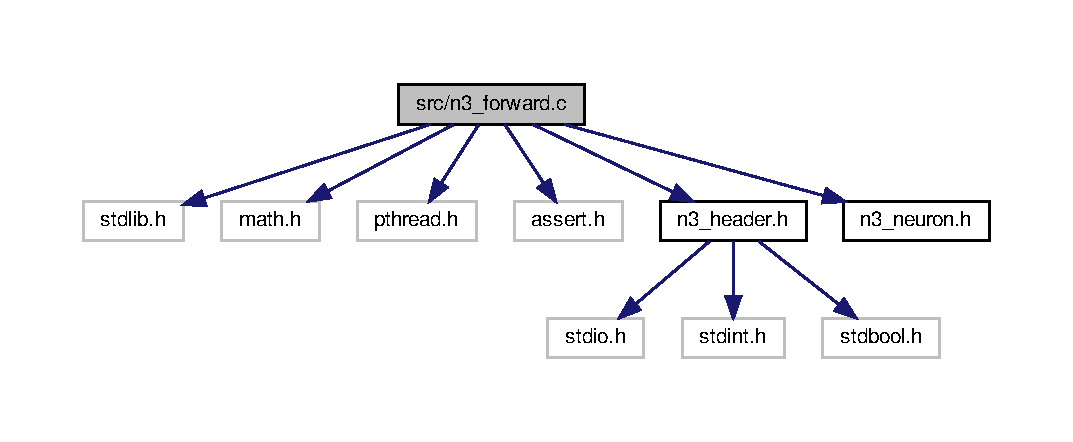
\includegraphics[width=350pt]{n3__forward_8c__incl}
\end{center}
\end{figure}
\subsection*{Data Structures}
\begin{DoxyCompactItemize}
\item 
struct \hyperlink{struct____n3l__forward__data}{\+\_\+\+\_\+n3l\+\_\+forward\+\_\+data}
\begin{DoxyCompactList}\small\item\em Internal struct to share data between threads. \end{DoxyCompactList}\end{DoxyCompactItemize}
\subsection*{Functions}
\begin{DoxyCompactItemize}
\item 
void $\ast$ \hyperlink{n3__forward_8c_af014464aaf6842d7da0ee6d1b1570ffe}{\+\_\+\+\_\+n3l\+\_\+forward\+\_\+activate} (void $\ast$arg)
\begin{DoxyCompactList}\small\item\em Internal function to execute the single neuron. \end{DoxyCompactList}\item 
void $\ast$ \hyperlink{n3__forward_8c_ac55d957c2a3b754387f5037e87317870}{\+\_\+\+\_\+n3l\+\_\+forward\+\_\+get\+\_\+outputs} (void $\ast$arg)
\begin{DoxyCompactList}\small\item\em Internal function to get outputs for the next layer\textquotesingle{}s neurons. \end{DoxyCompactList}\item 
double $\ast$ \hyperlink{n3__forward_8c_a658e97e1260b05ef3d286fbe93f11a40}{\+\_\+\+\_\+n3l\+\_\+forward\+\_\+layer} (\hyperlink{n3__header_8h_a9ee3a7104816bdb6222148cfe9ca8ad9}{N3\+L\+Layer} $\ast$layer, double $\ast$inputs)
\begin{DoxyCompactList}\small\item\em Internal function to execute forward propagation from the current layer to the next one. \end{DoxyCompactList}\item 
double $\ast$ \hyperlink{n3__forward_8c_abc37ac7f137db4d053e3b19ac8e6542a}{n3l\+\_\+forward\+\_\+propagation} (\hyperlink{structN3LNetwork}{N3\+L\+Network} $\ast$net)
\begin{DoxyCompactList}\small\item\em Execute forward propagation on the whole network. \end{DoxyCompactList}\end{DoxyCompactItemize}


\subsection{Detailed Description}
This file contains functions to forward the inputs provided to the outputs. 

\begin{DoxyAuthor}{Author}
Davide Francesco Merico 
\end{DoxyAuthor}


\subsection{Function Documentation}
\mbox{\Hypertarget{n3__forward_8c_af014464aaf6842d7da0ee6d1b1570ffe}\label{n3__forward_8c_af014464aaf6842d7da0ee6d1b1570ffe}} 
\index{n3\+\_\+forward.\+c@{n3\+\_\+forward.\+c}!\+\_\+\+\_\+n3l\+\_\+forward\+\_\+activate@{\+\_\+\+\_\+n3l\+\_\+forward\+\_\+activate}}
\index{\+\_\+\+\_\+n3l\+\_\+forward\+\_\+activate@{\+\_\+\+\_\+n3l\+\_\+forward\+\_\+activate}!n3\+\_\+forward.\+c@{n3\+\_\+forward.\+c}}
\subsubsection{\texorpdfstring{\+\_\+\+\_\+n3l\+\_\+forward\+\_\+activate()}{\_\_n3l\_forward\_activate()}}
{\footnotesize\ttfamily void $\ast$ \+\_\+\+\_\+n3l\+\_\+forward\+\_\+activate (\begin{DoxyParamCaption}\item[{void $\ast$}]{arg }\end{DoxyParamCaption})}



Internal function to execute the single neuron. 


\begin{DoxyParams}{Parameters}
{\em arg} & Current neuron to execute. \\
\hline
\end{DoxyParams}
\begin{DoxyReturn}{Returns}
N\+U\+LL.
\end{DoxyReturn}
\begin{DoxySeeAlso}{See also}
\hyperlink{n3__forward_8c_a658e97e1260b05ef3d286fbe93f11a40}{\+\_\+\+\_\+n3l\+\_\+forward\+\_\+layer}, \hyperlink{n3__forward_8c_ac55d957c2a3b754387f5037e87317870}{\+\_\+\+\_\+n3l\+\_\+forward\+\_\+get\+\_\+outputs}, \hyperlink{struct__n3l__neuron}{\+\_\+n3l\+\_\+neuron} 
\end{DoxySeeAlso}
\mbox{\Hypertarget{n3__forward_8c_ac55d957c2a3b754387f5037e87317870}\label{n3__forward_8c_ac55d957c2a3b754387f5037e87317870}} 
\index{n3\+\_\+forward.\+c@{n3\+\_\+forward.\+c}!\+\_\+\+\_\+n3l\+\_\+forward\+\_\+get\+\_\+outputs@{\+\_\+\+\_\+n3l\+\_\+forward\+\_\+get\+\_\+outputs}}
\index{\+\_\+\+\_\+n3l\+\_\+forward\+\_\+get\+\_\+outputs@{\+\_\+\+\_\+n3l\+\_\+forward\+\_\+get\+\_\+outputs}!n3\+\_\+forward.\+c@{n3\+\_\+forward.\+c}}
\subsubsection{\texorpdfstring{\+\_\+\+\_\+n3l\+\_\+forward\+\_\+get\+\_\+outputs()}{\_\_n3l\_forward\_get\_outputs()}}
{\footnotesize\ttfamily void $\ast$ \+\_\+\+\_\+n3l\+\_\+forward\+\_\+get\+\_\+outputs (\begin{DoxyParamCaption}\item[{void $\ast$}]{arg }\end{DoxyParamCaption})}



Internal function to get outputs for the next layer\textquotesingle{}s neurons. 


\begin{DoxyParams}{Parameters}
{\em arg} & thread data of type \hyperlink{struct____n3l__forward__data}{\+\_\+\+\_\+n3l\+\_\+forward\+\_\+data}. \\
\hline
\end{DoxyParams}
\begin{DoxyReturn}{Returns}
N\+U\+LL.
\end{DoxyReturn}
\begin{DoxySeeAlso}{See also}
\hyperlink{n3__forward_8c_a658e97e1260b05ef3d286fbe93f11a40}{\+\_\+\+\_\+n3l\+\_\+forward\+\_\+layer}, \hyperlink{n3__forward_8c_af014464aaf6842d7da0ee6d1b1570ffe}{\+\_\+\+\_\+n3l\+\_\+forward\+\_\+activate}, \hyperlink{struct____n3l__forward__data}{\+\_\+\+\_\+n3l\+\_\+forward\+\_\+data} 
\end{DoxySeeAlso}
\mbox{\Hypertarget{n3__forward_8c_a658e97e1260b05ef3d286fbe93f11a40}\label{n3__forward_8c_a658e97e1260b05ef3d286fbe93f11a40}} 
\index{n3\+\_\+forward.\+c@{n3\+\_\+forward.\+c}!\+\_\+\+\_\+n3l\+\_\+forward\+\_\+layer@{\+\_\+\+\_\+n3l\+\_\+forward\+\_\+layer}}
\index{\+\_\+\+\_\+n3l\+\_\+forward\+\_\+layer@{\+\_\+\+\_\+n3l\+\_\+forward\+\_\+layer}!n3\+\_\+forward.\+c@{n3\+\_\+forward.\+c}}
\subsubsection{\texorpdfstring{\+\_\+\+\_\+n3l\+\_\+forward\+\_\+layer()}{\_\_n3l\_forward\_layer()}}
{\footnotesize\ttfamily double $\ast$ \+\_\+\+\_\+n3l\+\_\+forward\+\_\+layer (\begin{DoxyParamCaption}\item[{\hyperlink{n3__header_8h_a9ee3a7104816bdb6222148cfe9ca8ad9}{N3\+L\+Layer} $\ast$}]{layer,  }\item[{double $\ast$}]{inputs }\end{DoxyParamCaption})}



Internal function to execute forward propagation from the current layer to the next one. 

This function first execute all neurons in the {\ttfamily layer} using concurrents threads. When all threads are executed, get the outputs for each neuron in the next layers.


\begin{DoxyParams}{Parameters}
{\em layer} & Current layer to execute. \\
\hline
{\em inputs} & Current layer inputs. \\
\hline
\end{DoxyParams}
\begin{DoxyReturn}{Returns}
Current layer outputs.
\end{DoxyReturn}
\begin{DoxySeeAlso}{See also}
\hyperlink{n3__forward_8c_abc37ac7f137db4d053e3b19ac8e6542a}{n3l\+\_\+forward\+\_\+propagation}, \hyperlink{n3__forward_8c_af014464aaf6842d7da0ee6d1b1570ffe}{\+\_\+\+\_\+n3l\+\_\+forward\+\_\+activate}, \hyperlink{n3__forward_8c_ac55d957c2a3b754387f5037e87317870}{\+\_\+\+\_\+n3l\+\_\+forward\+\_\+get\+\_\+outputs}, \hyperlink{struct__n3l__layer}{\+\_\+n3l\+\_\+layer} 
\end{DoxySeeAlso}
\mbox{\Hypertarget{n3__forward_8c_abc37ac7f137db4d053e3b19ac8e6542a}\label{n3__forward_8c_abc37ac7f137db4d053e3b19ac8e6542a}} 
\index{n3\+\_\+forward.\+c@{n3\+\_\+forward.\+c}!n3l\+\_\+forward\+\_\+propagation@{n3l\+\_\+forward\+\_\+propagation}}
\index{n3l\+\_\+forward\+\_\+propagation@{n3l\+\_\+forward\+\_\+propagation}!n3\+\_\+forward.\+c@{n3\+\_\+forward.\+c}}
\subsubsection{\texorpdfstring{n3l\+\_\+forward\+\_\+propagation()}{n3l\_forward\_propagation()}}
{\footnotesize\ttfamily double$\ast$ n3l\+\_\+forward\+\_\+propagation (\begin{DoxyParamCaption}\item[{\hyperlink{structN3LNetwork}{N3\+L\+Network} $\ast$}]{net }\end{DoxyParamCaption})}



Execute forward propagation on the whole network. 

\begin{DoxyNote}{Note}
The member {\ttfamily net-\/$>$inputs} must be initialized before calling this function. 
\end{DoxyNote}

\begin{DoxyParams}{Parameters}
{\em net} & Initialized network \\
\hline
\end{DoxyParams}
\begin{DoxyReturn}{Returns}
An array with the outputs evaluated. The array length is equal to the network output layer size. 
\end{DoxyReturn}
\begin{DoxyWarning}{Warning}
The returned array must be free manually calling free().
\end{DoxyWarning}
\begin{DoxySeeAlso}{See also}
n3l\+\_\+backward\+\_\+execute, \hyperlink{structN3LNetwork}{N3\+L\+Network}, \hyperlink{n3__forward_8c_a658e97e1260b05ef3d286fbe93f11a40}{\+\_\+\+\_\+n3l\+\_\+forward\+\_\+layer} 
\end{DoxySeeAlso}

\hypertarget{n3__header_8h}{}\section{src/n3\+\_\+header.h File Reference}
\label{n3__header_8h}\index{src/n3\+\_\+header.\+h@{src/n3\+\_\+header.\+h}}


This file contains types, enums and structs definitions.  


{\ttfamily \#include $<$stdio.\+h$>$}\newline
{\ttfamily \#include $<$stdint.\+h$>$}\newline
{\ttfamily \#include $<$stdbool.\+h$>$}\newline
Include dependency graph for n3\+\_\+header.\+h\+:\nopagebreak
\begin{figure}[H]
\begin{center}
\leavevmode
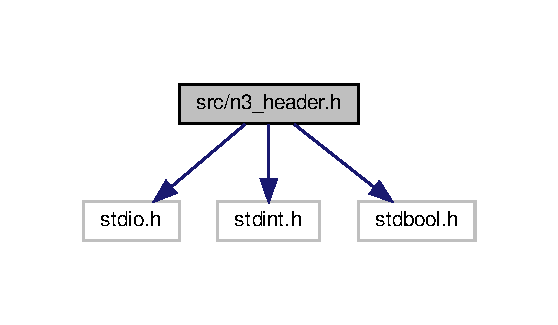
\includegraphics[width=268pt]{n3__header_8h__incl}
\end{center}
\end{figure}
This graph shows which files directly or indirectly include this file\+:
\nopagebreak
\begin{figure}[H]
\begin{center}
\leavevmode
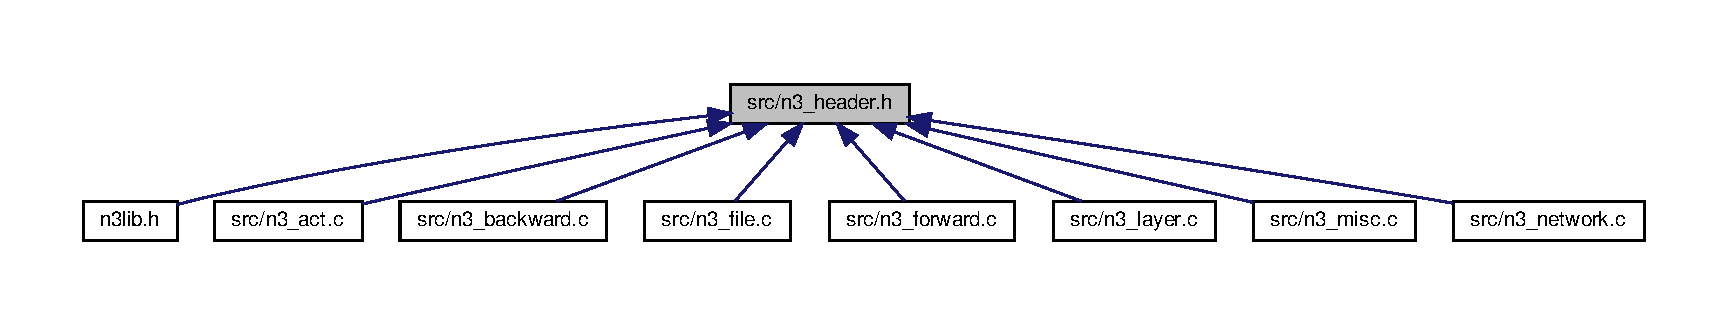
\includegraphics[width=350pt]{n3__header_8h__dep__incl}
\end{center}
\end{figure}
\subsection*{Data Structures}
\begin{DoxyCompactItemize}
\item 
struct \hyperlink{struct__n3l__weight}{\+\_\+n3l\+\_\+weight}
\begin{DoxyCompactList}\small\item\em Single Linked List which contains weight\textquotesingle{}s values. \end{DoxyCompactList}\item 
struct \hyperlink{struct__n3l__neuron}{\+\_\+n3l\+\_\+neuron}
\begin{DoxyCompactList}\small\item\em Double Linked List which contains neuron\textquotesingle{}s values. \end{DoxyCompactList}\item 
struct \hyperlink{struct__n3l__layer}{\+\_\+n3l\+\_\+layer}
\begin{DoxyCompactList}\small\item\em Double Linked List which contains layer\textquotesingle{}s values. \end{DoxyCompactList}\item 
struct \hyperlink{structN3LArgs}{N3\+L\+Args}
\begin{DoxyCompactList}\small\item\em Network arguments. \end{DoxyCompactList}\item 
struct \hyperlink{structN3LNetwork}{N3\+L\+Network}
\begin{DoxyCompactList}\small\item\em Network state. \end{DoxyCompactList}\end{DoxyCompactItemize}
\subsection*{Macros}
\begin{DoxyCompactItemize}
\item 
\mbox{\Hypertarget{n3__header_8h_a95bd80c66274b8f2dc5dd76bd547432e}\label{n3__header_8h_a95bd80c66274b8f2dc5dd76bd547432e}} 
\#define \hyperlink{n3__header_8h_a95bd80c66274b8f2dc5dd76bd547432e}{N3\+L\+\_\+\+V\+E\+R\+S\+I\+ON}~\char`\"{}2.\+0.\+0\char`\"{}
\begin{DoxyCompactList}\small\item\em N3 Library version. \end{DoxyCompactList}\end{DoxyCompactItemize}
\subsection*{Typedefs}
\begin{DoxyCompactItemize}
\item 
typedef double($\ast$ \hyperlink{n3__header_8h_afb10e6f7012513b51225a4d3add36cae}{N3\+L\+Act}) (double)
\begin{DoxyCompactList}\small\item\em Pointer to an activation function. \end{DoxyCompactList}\item 
typedef double($\ast$ \hyperlink{n3__header_8h_ab3b7d8e984e9ad2e4d5e7cbe433ad572}{N3\+L\+Weight\+Generator}) (void $\ast$)
\begin{DoxyCompactList}\small\item\em Pointer to a function to get the network weights. \end{DoxyCompactList}\item 
typedef struct \hyperlink{struct__n3l__weight}{\+\_\+n3l\+\_\+weight} \hyperlink{n3__header_8h_ac37c67a24ec253f5cd205cbc981922ca}{N3\+L\+Weight}
\begin{DoxyCompactList}\small\item\em Single Linked List which contains weight\textquotesingle{}s values. \end{DoxyCompactList}\item 
typedef struct \hyperlink{struct__n3l__neuron}{\+\_\+n3l\+\_\+neuron} \hyperlink{n3__header_8h_a621b1df037f351bd3542298933e5799a}{N3\+L\+Neuron}
\begin{DoxyCompactList}\small\item\em Double Linked List which contains neuron\textquotesingle{}s values. \end{DoxyCompactList}\item 
typedef struct \hyperlink{struct__n3l__layer}{\+\_\+n3l\+\_\+layer} \hyperlink{n3__header_8h_a9ee3a7104816bdb6222148cfe9ca8ad9}{N3\+L\+Layer}
\begin{DoxyCompactList}\small\item\em Double Linked List which contains layer\textquotesingle{}s values. \end{DoxyCompactList}\end{DoxyCompactItemize}
\subsection*{Enumerations}
\begin{DoxyCompactItemize}
\item 
enum \hyperlink{n3__header_8h_a1040baea07fec4d26d25641f75e892c5}{N3\+L\+Layer\+Type} \{ \hyperlink{n3__header_8h_a1040baea07fec4d26d25641f75e892c5aab750c92dd8be2c9e55ed46d05daadb4}{N3\+L\+Input\+Layer} = 0, 
\hyperlink{n3__header_8h_a1040baea07fec4d26d25641f75e892c5abe1288f7415a2918a6bd13c36d84ac11}{N3\+L\+Hidden\+Layer}, 
\hyperlink{n3__header_8h_a1040baea07fec4d26d25641f75e892c5a8251417b1ede207c8506218740c9f8b1}{N3\+L\+Output\+Layer}
 \}\begin{DoxyCompactList}\small\item\em Identify the layer type. \end{DoxyCompactList}
\item 
enum \hyperlink{n3__header_8h_a3118e8995213ca26bd388c3d94cd8056}{N3\+L\+Act\+Type} \{ \newline
\hyperlink{n3__header_8h_a3118e8995213ca26bd388c3d94cd8056a43a8cba04b86be267aa4a9705ccb74d2}{N3\+L\+Custom} = -\/1, 
\hyperlink{n3__header_8h_a3118e8995213ca26bd388c3d94cd8056af6be5bcaf85e8fc974b3fc20dad32d18}{N3\+L\+None} = 0, 
\hyperlink{n3__header_8h_a3118e8995213ca26bd388c3d94cd8056a58c090ee14de5def02bd6aaa27af7888}{N3\+L\+Sigmoid}, 
\hyperlink{n3__header_8h_a3118e8995213ca26bd388c3d94cd8056a7fcd20d1c210fa86c867f386b809c109}{N3\+L\+Tanh}, 
\newline
\hyperlink{n3__header_8h_a3118e8995213ca26bd388c3d94cd8056ad23c37f3c19c399a7766983c87ca6794}{N3\+L\+Relu}, 
\hyperlink{n3__header_8h_a3118e8995213ca26bd388c3d94cd8056a6ba1b3ad5fc8cc7b017b76ad770daa1e}{N3\+L\+Identity}, 
\hyperlink{n3__header_8h_a3118e8995213ca26bd388c3d94cd8056a6745742e74cf12f866a4093e5a61156d}{N3\+L\+Leaky\+Relu}, 
\hyperlink{n3__header_8h_a3118e8995213ca26bd388c3d94cd8056ad0d9ce7eb6b4357996fe7a6ff2e972c8}{N3\+L\+Soft\+Plus}, 
\newline
\hyperlink{n3__header_8h_a3118e8995213ca26bd388c3d94cd8056aa399b22b7aa19e9544c71fe611f99b29}{N3\+L\+Soft\+Sign}, 
\hyperlink{n3__header_8h_a3118e8995213ca26bd388c3d94cd8056a8cdff3364dcd3d15c824a28d1dd4b89b}{N3\+L\+Swish}
 \}\begin{DoxyCompactList}\small\item\em Activation function type. \end{DoxyCompactList}
\end{DoxyCompactItemize}


\subsection{Detailed Description}
This file contains types, enums and structs definitions. 

\begin{DoxyAuthor}{Author}
Davide Francesco Merico 
\end{DoxyAuthor}


\subsection{Typedef Documentation}
\mbox{\Hypertarget{n3__header_8h_afb10e6f7012513b51225a4d3add36cae}\label{n3__header_8h_afb10e6f7012513b51225a4d3add36cae}} 
\index{n3\+\_\+header.\+h@{n3\+\_\+header.\+h}!N3\+L\+Act@{N3\+L\+Act}}
\index{N3\+L\+Act@{N3\+L\+Act}!n3\+\_\+header.\+h@{n3\+\_\+header.\+h}}
\subsubsection{\texorpdfstring{N3\+L\+Act}{N3LAct}}
{\footnotesize\ttfamily typedef double($\ast$ N3\+L\+Act) (double)}



Pointer to an activation function. 

\begin{DoxySeeAlso}{See also}
\hyperlink{n3__act_8c_af9034678bae2b94ebcf0d9b2ac5cfcb7}{n3l\+\_\+act}, \hyperlink{n3__act_8c_a9253520cb5a58edf61f04997c3161f21}{n3l\+\_\+act\+\_\+prime}, \hyperlink{struct__n3l__neuron}{\+\_\+n3l\+\_\+neuron} 
\end{DoxySeeAlso}
\mbox{\Hypertarget{n3__header_8h_a9ee3a7104816bdb6222148cfe9ca8ad9}\label{n3__header_8h_a9ee3a7104816bdb6222148cfe9ca8ad9}} 
\index{n3\+\_\+header.\+h@{n3\+\_\+header.\+h}!N3\+L\+Layer@{N3\+L\+Layer}}
\index{N3\+L\+Layer@{N3\+L\+Layer}!n3\+\_\+header.\+h@{n3\+\_\+header.\+h}}
\subsubsection{\texorpdfstring{N3\+L\+Layer}{N3LLayer}}
{\footnotesize\ttfamily typedef struct \hyperlink{struct__n3l__layer}{\+\_\+n3l\+\_\+layer}  \hyperlink{n3__header_8h_a9ee3a7104816bdb6222148cfe9ca8ad9}{N3\+L\+Layer}}



Double Linked List which contains layer\textquotesingle{}s values. 

The list is built by \hyperlink{n3__network_8c_a5f87e1efebd658dd55d7d2ca1768bdba}{n3l\+\_\+network\+\_\+build()} or \hyperlink{n3__file_8c_a4fef76548ed87845dceafaa9527a83d0}{n3l\+\_\+file\+\_\+import\+\_\+network()}.

\begin{DoxySeeAlso}{See also}
\hyperlink{struct__n3l__neuron}{\+\_\+n3l\+\_\+neuron}, \hyperlink{structN3LNetwork}{N3\+L\+Network}, \hyperlink{n3__layer_8c_a135215adb7cf8420293fd4ebd7049655}{n3l\+\_\+layer\+\_\+build}, \hyperlink{n3__layer_8c_ab06afb58d55be21a00bde5ee840f6425}{n3l\+\_\+layer\+\_\+count}, \hyperlink{n3__layer_8c_ad58e1630c1b7fc5da03d54cf63c394d9}{n3l\+\_\+layer\+\_\+free} 
\end{DoxySeeAlso}
\mbox{\Hypertarget{n3__header_8h_a621b1df037f351bd3542298933e5799a}\label{n3__header_8h_a621b1df037f351bd3542298933e5799a}} 
\index{n3\+\_\+header.\+h@{n3\+\_\+header.\+h}!N3\+L\+Neuron@{N3\+L\+Neuron}}
\index{N3\+L\+Neuron@{N3\+L\+Neuron}!n3\+\_\+header.\+h@{n3\+\_\+header.\+h}}
\subsubsection{\texorpdfstring{N3\+L\+Neuron}{N3LNeuron}}
{\footnotesize\ttfamily typedef struct \hyperlink{struct__n3l__neuron}{\+\_\+n3l\+\_\+neuron}  \hyperlink{n3__header_8h_a621b1df037f351bd3542298933e5799a}{N3\+L\+Neuron}}



Double Linked List which contains neuron\textquotesingle{}s values. 

The list is built by \hyperlink{n3__network_8c_a5f87e1efebd658dd55d7d2ca1768bdba}{n3l\+\_\+network\+\_\+build()} or \hyperlink{n3__file_8c_a4fef76548ed87845dceafaa9527a83d0}{n3l\+\_\+file\+\_\+import\+\_\+network()}.

\begin{DoxySeeAlso}{See also}
\hyperlink{struct__n3l__layer}{\+\_\+n3l\+\_\+layer}, \hyperlink{struct__n3l__weight}{\+\_\+n3l\+\_\+weight}, n3l\+\_\+neuron\+\_\+build, n3l\+\_\+neuron\+\_\+count, n3l\+\_\+neuron\+\_\+free 
\end{DoxySeeAlso}
\mbox{\Hypertarget{n3__header_8h_ac37c67a24ec253f5cd205cbc981922ca}\label{n3__header_8h_ac37c67a24ec253f5cd205cbc981922ca}} 
\index{n3\+\_\+header.\+h@{n3\+\_\+header.\+h}!N3\+L\+Weight@{N3\+L\+Weight}}
\index{N3\+L\+Weight@{N3\+L\+Weight}!n3\+\_\+header.\+h@{n3\+\_\+header.\+h}}
\subsubsection{\texorpdfstring{N3\+L\+Weight}{N3LWeight}}
{\footnotesize\ttfamily typedef struct \hyperlink{struct__n3l__weight}{\+\_\+n3l\+\_\+weight}  \hyperlink{n3__header_8h_ac37c67a24ec253f5cd205cbc981922ca}{N3\+L\+Weight}}



Single Linked List which contains weight\textquotesingle{}s values. 

The list is built by \hyperlink{n3__network_8c_a5f87e1efebd658dd55d7d2ca1768bdba}{n3l\+\_\+network\+\_\+build()} or \hyperlink{n3__file_8c_a4fef76548ed87845dceafaa9527a83d0}{n3l\+\_\+file\+\_\+import\+\_\+network()}.

\begin{DoxySeeAlso}{See also}
\hyperlink{struct__n3l__neuron}{\+\_\+n3l\+\_\+neuron}, n3l\+\_\+neuron\+\_\+get\+\_\+weight, n3l\+\_\+neuron\+\_\+count\+\_\+weights, n3l\+\_\+neuron\+\_\+build\+\_\+weights 
\end{DoxySeeAlso}
\mbox{\Hypertarget{n3__header_8h_ab3b7d8e984e9ad2e4d5e7cbe433ad572}\label{n3__header_8h_ab3b7d8e984e9ad2e4d5e7cbe433ad572}} 
\index{n3\+\_\+header.\+h@{n3\+\_\+header.\+h}!N3\+L\+Weight\+Generator@{N3\+L\+Weight\+Generator}}
\index{N3\+L\+Weight\+Generator@{N3\+L\+Weight\+Generator}!n3\+\_\+header.\+h@{n3\+\_\+header.\+h}}
\subsubsection{\texorpdfstring{N3\+L\+Weight\+Generator}{N3LWeightGenerator}}
{\footnotesize\ttfamily typedef double($\ast$ N3\+L\+Weight\+Generator) (void $\ast$)}



Pointer to a function to get the network weights. 

Used to get weights when a network is imported or built.

\begin{DoxySeeAlso}{See also}
\hyperlink{n3__misc_8c_ad000cb3ea3bb9c116899973c4c382c64}{n3l\+\_\+misc\+\_\+rnd\+\_\+wp1}, \hyperlink{n3__misc_8c_a20bef1a0eb58f93a1cd935ace0af28a8}{n3l\+\_\+misc\+\_\+rnd\+\_\+wn1}, \hyperlink{n3__misc_8c_a31bb0c8231fc4206075182808c2b0348}{n3l\+\_\+misc\+\_\+rnd\+\_\+wpn1}, \hyperlink{n3__file_8c_a78616ce6ffbb8218a169905de93abaaa}{\+\_\+\+\_\+n3l\+\_\+get\+\_\+weight\+\_\+from\+\_\+file} 
\end{DoxySeeAlso}


\subsection{Enumeration Type Documentation}
\mbox{\Hypertarget{n3__header_8h_a3118e8995213ca26bd388c3d94cd8056}\label{n3__header_8h_a3118e8995213ca26bd388c3d94cd8056}} 
\index{n3\+\_\+header.\+h@{n3\+\_\+header.\+h}!N3\+L\+Act\+Type@{N3\+L\+Act\+Type}}
\index{N3\+L\+Act\+Type@{N3\+L\+Act\+Type}!n3\+\_\+header.\+h@{n3\+\_\+header.\+h}}
\subsubsection{\texorpdfstring{N3\+L\+Act\+Type}{N3LActType}}
{\footnotesize\ttfamily enum \hyperlink{n3__header_8h_a3118e8995213ca26bd388c3d94cd8056}{N3\+L\+Act\+Type}}



Activation function type. 

\begin{DoxySeeAlso}{See also}
\hyperlink{n3__act_8c_af9034678bae2b94ebcf0d9b2ac5cfcb7}{n3l\+\_\+act}, \hyperlink{n3__act_8c_a9253520cb5a58edf61f04997c3161f21}{n3l\+\_\+act\+\_\+prime}, \hyperlink{struct__n3l__neuron}{\+\_\+n3l\+\_\+neuron} 
\end{DoxySeeAlso}
\begin{DoxyEnumFields}{Enumerator}
\raisebox{\heightof{T}}[0pt][0pt]{\index{N3\+L\+Custom@{N3\+L\+Custom}!n3\+\_\+header.\+h@{n3\+\_\+header.\+h}}\index{n3\+\_\+header.\+h@{n3\+\_\+header.\+h}!N3\+L\+Custom@{N3\+L\+Custom}}}\mbox{\Hypertarget{n3__header_8h_a3118e8995213ca26bd388c3d94cd8056a43a8cba04b86be267aa4a9705ccb74d2}\label{n3__header_8h_a3118e8995213ca26bd388c3d94cd8056a43a8cba04b86be267aa4a9705ccb74d2}} 
N3\+L\+Custom&Custom activation function. \begin{DoxySeeAlso}{See also}
\hyperlink{n3__layer_8c_a097eadb210e490788ebf2a7c1c614c6f}{n3l\+\_\+layer\+\_\+set\+\_\+custom\+\_\+act}, n3l\+\_\+neuron\+\_\+set\+\_\+custom\+\_\+act 
\end{DoxySeeAlso}
\\
\hline

\raisebox{\heightof{T}}[0pt][0pt]{\index{N3\+L\+None@{N3\+L\+None}!n3\+\_\+header.\+h@{n3\+\_\+header.\+h}}\index{n3\+\_\+header.\+h@{n3\+\_\+header.\+h}!N3\+L\+None@{N3\+L\+None}}}\mbox{\Hypertarget{n3__header_8h_a3118e8995213ca26bd388c3d94cd8056af6be5bcaf85e8fc974b3fc20dad32d18}\label{n3__header_8h_a3118e8995213ca26bd388c3d94cd8056af6be5bcaf85e8fc974b3fc20dad32d18}} 
N3\+L\+None&No activation function. \begin{DoxySeeAlso}{See also}
\hyperlink{n3__act_8c_a8dc073371b15e2574897762b54f9326c}{n3l\+\_\+act\+\_\+none} 
\end{DoxySeeAlso}
\\
\hline

\raisebox{\heightof{T}}[0pt][0pt]{\index{N3\+L\+Sigmoid@{N3\+L\+Sigmoid}!n3\+\_\+header.\+h@{n3\+\_\+header.\+h}}\index{n3\+\_\+header.\+h@{n3\+\_\+header.\+h}!N3\+L\+Sigmoid@{N3\+L\+Sigmoid}}}\mbox{\Hypertarget{n3__header_8h_a3118e8995213ca26bd388c3d94cd8056a58c090ee14de5def02bd6aaa27af7888}\label{n3__header_8h_a3118e8995213ca26bd388c3d94cd8056a58c090ee14de5def02bd6aaa27af7888}} 
N3\+L\+Sigmoid&Sigmoid activation function. \begin{DoxySeeAlso}{See also}
\hyperlink{n3__act_8c_ad01dde283500e1fbac8d916967bfd883}{n3l\+\_\+act\+\_\+sigmoid} 
\end{DoxySeeAlso}
\\
\hline

\raisebox{\heightof{T}}[0pt][0pt]{\index{N3\+L\+Tanh@{N3\+L\+Tanh}!n3\+\_\+header.\+h@{n3\+\_\+header.\+h}}\index{n3\+\_\+header.\+h@{n3\+\_\+header.\+h}!N3\+L\+Tanh@{N3\+L\+Tanh}}}\mbox{\Hypertarget{n3__header_8h_a3118e8995213ca26bd388c3d94cd8056a7fcd20d1c210fa86c867f386b809c109}\label{n3__header_8h_a3118e8995213ca26bd388c3d94cd8056a7fcd20d1c210fa86c867f386b809c109}} 
N3\+L\+Tanh&Tanh activation function. \begin{DoxySeeAlso}{See also}
\hyperlink{n3__act_8c_aa05576ce02d1c18c0af9f042d1068c7a}{n3l\+\_\+act\+\_\+tanh} 
\end{DoxySeeAlso}
\\
\hline

\raisebox{\heightof{T}}[0pt][0pt]{\index{N3\+L\+Relu@{N3\+L\+Relu}!n3\+\_\+header.\+h@{n3\+\_\+header.\+h}}\index{n3\+\_\+header.\+h@{n3\+\_\+header.\+h}!N3\+L\+Relu@{N3\+L\+Relu}}}\mbox{\Hypertarget{n3__header_8h_a3118e8995213ca26bd388c3d94cd8056ad23c37f3c19c399a7766983c87ca6794}\label{n3__header_8h_a3118e8995213ca26bd388c3d94cd8056ad23c37f3c19c399a7766983c87ca6794}} 
N3\+L\+Relu&Re\+LU activation function. \begin{DoxySeeAlso}{See also}
\hyperlink{n3__act_8c_a07a8cded25f1d3b726053b50cba78eb0}{n3l\+\_\+act\+\_\+relu} 
\end{DoxySeeAlso}
\\
\hline

\raisebox{\heightof{T}}[0pt][0pt]{\index{N3\+L\+Identity@{N3\+L\+Identity}!n3\+\_\+header.\+h@{n3\+\_\+header.\+h}}\index{n3\+\_\+header.\+h@{n3\+\_\+header.\+h}!N3\+L\+Identity@{N3\+L\+Identity}}}\mbox{\Hypertarget{n3__header_8h_a3118e8995213ca26bd388c3d94cd8056a6ba1b3ad5fc8cc7b017b76ad770daa1e}\label{n3__header_8h_a3118e8995213ca26bd388c3d94cd8056a6ba1b3ad5fc8cc7b017b76ad770daa1e}} 
N3\+L\+Identity&Identity activation function. \begin{DoxySeeAlso}{See also}
\hyperlink{n3__act_8c_a066f6fed961da89043b1b496aa5ac6d0}{n3l\+\_\+act\+\_\+identity} 
\end{DoxySeeAlso}
\\
\hline

\raisebox{\heightof{T}}[0pt][0pt]{\index{N3\+L\+Leaky\+Relu@{N3\+L\+Leaky\+Relu}!n3\+\_\+header.\+h@{n3\+\_\+header.\+h}}\index{n3\+\_\+header.\+h@{n3\+\_\+header.\+h}!N3\+L\+Leaky\+Relu@{N3\+L\+Leaky\+Relu}}}\mbox{\Hypertarget{n3__header_8h_a3118e8995213ca26bd388c3d94cd8056a6745742e74cf12f866a4093e5a61156d}\label{n3__header_8h_a3118e8995213ca26bd388c3d94cd8056a6745742e74cf12f866a4093e5a61156d}} 
N3\+L\+Leaky\+Relu&Leaky Re\+LU activation function. \begin{DoxySeeAlso}{See also}
\hyperlink{n3__act_8c_a2091491a8d0155701b6170c324b52eef}{n3l\+\_\+act\+\_\+leaky\+\_\+relu} 
\end{DoxySeeAlso}
\\
\hline

\raisebox{\heightof{T}}[0pt][0pt]{\index{N3\+L\+Soft\+Plus@{N3\+L\+Soft\+Plus}!n3\+\_\+header.\+h@{n3\+\_\+header.\+h}}\index{n3\+\_\+header.\+h@{n3\+\_\+header.\+h}!N3\+L\+Soft\+Plus@{N3\+L\+Soft\+Plus}}}\mbox{\Hypertarget{n3__header_8h_a3118e8995213ca26bd388c3d94cd8056ad0d9ce7eb6b4357996fe7a6ff2e972c8}\label{n3__header_8h_a3118e8995213ca26bd388c3d94cd8056ad0d9ce7eb6b4357996fe7a6ff2e972c8}} 
N3\+L\+Soft\+Plus&Soft\+Plus activation function. \begin{DoxySeeAlso}{See also}
\hyperlink{n3__act_8c_ab678727eab04c73e227d0511f10da9ab}{n3l\+\_\+act\+\_\+softplus} 
\end{DoxySeeAlso}
\\
\hline

\raisebox{\heightof{T}}[0pt][0pt]{\index{N3\+L\+Soft\+Sign@{N3\+L\+Soft\+Sign}!n3\+\_\+header.\+h@{n3\+\_\+header.\+h}}\index{n3\+\_\+header.\+h@{n3\+\_\+header.\+h}!N3\+L\+Soft\+Sign@{N3\+L\+Soft\+Sign}}}\mbox{\Hypertarget{n3__header_8h_a3118e8995213ca26bd388c3d94cd8056aa399b22b7aa19e9544c71fe611f99b29}\label{n3__header_8h_a3118e8995213ca26bd388c3d94cd8056aa399b22b7aa19e9544c71fe611f99b29}} 
N3\+L\+Soft\+Sign&Soft\+Sign activation function. \begin{DoxySeeAlso}{See also}
\hyperlink{n3__act_8c_a9e9cd6045617a4063602ccd9e94281bf}{n3l\+\_\+act\+\_\+softsign} 
\end{DoxySeeAlso}
\\
\hline

\raisebox{\heightof{T}}[0pt][0pt]{\index{N3\+L\+Swish@{N3\+L\+Swish}!n3\+\_\+header.\+h@{n3\+\_\+header.\+h}}\index{n3\+\_\+header.\+h@{n3\+\_\+header.\+h}!N3\+L\+Swish@{N3\+L\+Swish}}}\mbox{\Hypertarget{n3__header_8h_a3118e8995213ca26bd388c3d94cd8056a8cdff3364dcd3d15c824a28d1dd4b89b}\label{n3__header_8h_a3118e8995213ca26bd388c3d94cd8056a8cdff3364dcd3d15c824a28d1dd4b89b}} 
N3\+L\+Swish&Swish activation function. \begin{DoxySeeAlso}{See also}
\hyperlink{n3__act_8c_a64fdb17c0915027691ad0b1340bdb1af}{n3l\+\_\+act\+\_\+swish} 
\end{DoxySeeAlso}
\\
\hline

\end{DoxyEnumFields}
\mbox{\Hypertarget{n3__header_8h_a1040baea07fec4d26d25641f75e892c5}\label{n3__header_8h_a1040baea07fec4d26d25641f75e892c5}} 
\index{n3\+\_\+header.\+h@{n3\+\_\+header.\+h}!N3\+L\+Layer\+Type@{N3\+L\+Layer\+Type}}
\index{N3\+L\+Layer\+Type@{N3\+L\+Layer\+Type}!n3\+\_\+header.\+h@{n3\+\_\+header.\+h}}
\subsubsection{\texorpdfstring{N3\+L\+Layer\+Type}{N3LLayerType}}
{\footnotesize\ttfamily enum \hyperlink{n3__header_8h_a1040baea07fec4d26d25641f75e892c5}{N3\+L\+Layer\+Type}}



Identify the layer type. 

\begin{DoxySeeAlso}{See also}
\hyperlink{struct__n3l__layer}{\+\_\+n3l\+\_\+layer} 
\end{DoxySeeAlso}
\begin{DoxyEnumFields}{Enumerator}
\raisebox{\heightof{T}}[0pt][0pt]{\index{N3\+L\+Input\+Layer@{N3\+L\+Input\+Layer}!n3\+\_\+header.\+h@{n3\+\_\+header.\+h}}\index{n3\+\_\+header.\+h@{n3\+\_\+header.\+h}!N3\+L\+Input\+Layer@{N3\+L\+Input\+Layer}}}\mbox{\Hypertarget{n3__header_8h_a1040baea07fec4d26d25641f75e892c5aab750c92dd8be2c9e55ed46d05daadb4}\label{n3__header_8h_a1040baea07fec4d26d25641f75e892c5aab750c92dd8be2c9e55ed46d05daadb4}} 
N3\+L\+Input\+Layer&Input layer, usually this type of layer doesn\textquotesingle{}t have a previous layer linked. \\
\hline

\raisebox{\heightof{T}}[0pt][0pt]{\index{N3\+L\+Hidden\+Layer@{N3\+L\+Hidden\+Layer}!n3\+\_\+header.\+h@{n3\+\_\+header.\+h}}\index{n3\+\_\+header.\+h@{n3\+\_\+header.\+h}!N3\+L\+Hidden\+Layer@{N3\+L\+Hidden\+Layer}}}\mbox{\Hypertarget{n3__header_8h_a1040baea07fec4d26d25641f75e892c5abe1288f7415a2918a6bd13c36d84ac11}\label{n3__header_8h_a1040baea07fec4d26d25641f75e892c5abe1288f7415a2918a6bd13c36d84ac11}} 
N3\+L\+Hidden\+Layer&Hidden Layer, usually have both previous and next layer linked. \\
\hline

\raisebox{\heightof{T}}[0pt][0pt]{\index{N3\+L\+Output\+Layer@{N3\+L\+Output\+Layer}!n3\+\_\+header.\+h@{n3\+\_\+header.\+h}}\index{n3\+\_\+header.\+h@{n3\+\_\+header.\+h}!N3\+L\+Output\+Layer@{N3\+L\+Output\+Layer}}}\mbox{\Hypertarget{n3__header_8h_a1040baea07fec4d26d25641f75e892c5a8251417b1ede207c8506218740c9f8b1}\label{n3__header_8h_a1040baea07fec4d26d25641f75e892c5a8251417b1ede207c8506218740c9f8b1}} 
N3\+L\+Output\+Layer&Output Layer, usually this type of layer doesn\textquotesingle{}t have a next layer linked. \\
\hline

\end{DoxyEnumFields}

\hypertarget{n3__layer_8c}{}\section{src/n3\+\_\+layer.c File Reference}
\label{n3__layer_8c}\index{src/n3\+\_\+layer.\+c@{src/n3\+\_\+layer.\+c}}


This file contains functions to work with N3\+Layers.  


{\ttfamily \#include $<$stdlib.\+h$>$}\newline
{\ttfamily \#include \char`\"{}n3\+\_\+header.\+h\char`\"{}}\newline
{\ttfamily \#include \char`\"{}n3\+\_\+neuron.\+h\char`\"{}}\newline
Include dependency graph for n3\+\_\+layer.\+c\+:\nopagebreak
\begin{figure}[H]
\begin{center}
\leavevmode
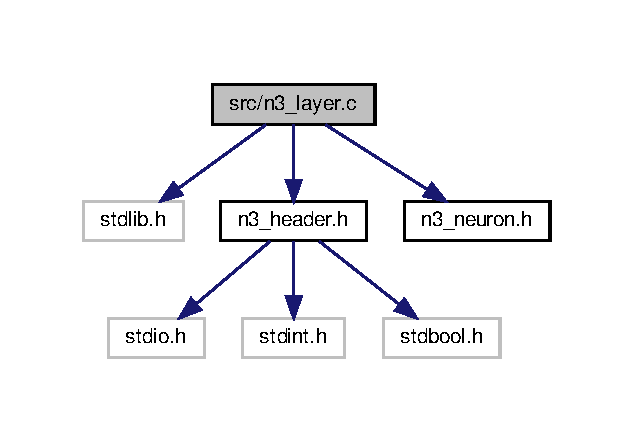
\includegraphics[width=304pt]{n3__layer_8c__incl}
\end{center}
\end{figure}
\subsection*{Functions}
\begin{DoxyCompactItemize}
\item 
\hyperlink{n3__header_8h_a9ee3a7104816bdb6222148cfe9ca8ad9}{N3\+L\+Layer} $\ast$ \hyperlink{n3__layer_8c_a135215adb7cf8420293fd4ebd7049655}{n3l\+\_\+layer\+\_\+build} (\hyperlink{n3__header_8h_a1040baea07fec4d26d25641f75e892c5}{N3\+L\+Layer\+Type} ltype)
\begin{DoxyCompactList}\small\item\em Build a layer. \end{DoxyCompactList}\item 
\hyperlink{n3__header_8h_a9ee3a7104816bdb6222148cfe9ca8ad9}{N3\+L\+Layer} $\ast$ \hyperlink{n3__layer_8c_ae58fb96c07e37c8645e8fd9f2a76c725}{n3l\+\_\+layer\+\_\+build\+\_\+after} (\hyperlink{n3__header_8h_a9ee3a7104816bdb6222148cfe9ca8ad9}{N3\+L\+Layer} $\ast$prev, \hyperlink{n3__header_8h_a1040baea07fec4d26d25641f75e892c5}{N3\+L\+Layer\+Type} ltype)
\begin{DoxyCompactList}\small\item\em Build a layer linked to a previous one. \end{DoxyCompactList}\item 
\hyperlink{n3__header_8h_a9ee3a7104816bdb6222148cfe9ca8ad9}{N3\+L\+Layer} $\ast$ \hyperlink{n3__layer_8c_a34b79476ceb642057989ab8691b2ce1d}{n3l\+\_\+layer\+\_\+build\+\_\+before} (\hyperlink{n3__header_8h_a9ee3a7104816bdb6222148cfe9ca8ad9}{N3\+L\+Layer} $\ast$next, \hyperlink{n3__header_8h_a1040baea07fec4d26d25641f75e892c5}{N3\+L\+Layer\+Type} ltype)
\begin{DoxyCompactList}\small\item\em Build a layer linked to a next one. \end{DoxyCompactList}\item 
uint64\+\_\+t \hyperlink{n3__layer_8c_ab06afb58d55be21a00bde5ee840f6425}{n3l\+\_\+layer\+\_\+count} (\hyperlink{n3__header_8h_a9ee3a7104816bdb6222148cfe9ca8ad9}{N3\+L\+Layer} $\ast$head)
\begin{DoxyCompactList}\small\item\em Count the layers from the layer passed as argument. \end{DoxyCompactList}\item 
void \hyperlink{n3__layer_8c_ad58e1630c1b7fc5da03d54cf63c394d9}{n3l\+\_\+layer\+\_\+free} (\hyperlink{n3__header_8h_a9ee3a7104816bdb6222148cfe9ca8ad9}{N3\+L\+Layer} $\ast$layer)
\begin{DoxyCompactList}\small\item\em Free the layer\textquotesingle{}s allocated memory. \end{DoxyCompactList}\item 
void \hyperlink{n3__layer_8c_a097eadb210e490788ebf2a7c1c614c6f}{n3l\+\_\+layer\+\_\+set\+\_\+custom\+\_\+act} (\hyperlink{n3__header_8h_a9ee3a7104816bdb6222148cfe9ca8ad9}{N3\+L\+Layer} $\ast$layer, \hyperlink{n3__header_8h_afb10e6f7012513b51225a4d3add36cae}{N3\+L\+Act} act, \hyperlink{n3__header_8h_afb10e6f7012513b51225a4d3add36cae}{N3\+L\+Act} prime, bool ignore\+\_\+bias)
\begin{DoxyCompactList}\small\item\em Set custom activation functions to the layer\textquotesingle{}s neurons. \end{DoxyCompactList}\end{DoxyCompactItemize}


\subsection{Detailed Description}
This file contains functions to work with N3\+Layers. 

\begin{DoxyAuthor}{Author}
Davide Francesco Merico 
\end{DoxyAuthor}
\begin{DoxyNote}{Note}
You may not use these functions directly but use functions like \hyperlink{n3__network_8c_a5f87e1efebd658dd55d7d2ca1768bdba}{n3l\+\_\+network\+\_\+build()}, \hyperlink{n3__network_8c_a327ffd586b67f586743d72a146c4ea95}{n3l\+\_\+network\+\_\+free()}, \hyperlink{n3__file_8c_a4fef76548ed87845dceafaa9527a83d0}{n3l\+\_\+file\+\_\+import\+\_\+network()}, etc.. 
\end{DoxyNote}


\subsection{Function Documentation}
\mbox{\Hypertarget{n3__layer_8c_a135215adb7cf8420293fd4ebd7049655}\label{n3__layer_8c_a135215adb7cf8420293fd4ebd7049655}} 
\index{n3\+\_\+layer.\+c@{n3\+\_\+layer.\+c}!n3l\+\_\+layer\+\_\+build@{n3l\+\_\+layer\+\_\+build}}
\index{n3l\+\_\+layer\+\_\+build@{n3l\+\_\+layer\+\_\+build}!n3\+\_\+layer.\+c@{n3\+\_\+layer.\+c}}
\subsubsection{\texorpdfstring{n3l\+\_\+layer\+\_\+build()}{n3l\_layer\_build()}}
{\footnotesize\ttfamily \hyperlink{n3__header_8h_a9ee3a7104816bdb6222148cfe9ca8ad9}{N3\+L\+Layer}$\ast$ n3l\+\_\+layer\+\_\+build (\begin{DoxyParamCaption}\item[{\hyperlink{n3__header_8h_a1040baea07fec4d26d25641f75e892c5}{N3\+L\+Layer\+Type}}]{ltype }\end{DoxyParamCaption})}



Build a layer. 


\begin{DoxyParams}{Parameters}
{\em ltype} & Layer type. \\
\hline
\end{DoxyParams}
\begin{DoxyReturn}{Returns}
The new built layer of type {\ttfamily ltype}.
\end{DoxyReturn}
\begin{DoxyNote}{Note}
References to neurons or others layers are set to N\+U\+LL. 
\end{DoxyNote}
\begin{DoxySeeAlso}{See also}
\hyperlink{n3__layer_8c_ae58fb96c07e37c8645e8fd9f2a76c725}{n3l\+\_\+layer\+\_\+build\+\_\+after}, \hyperlink{n3__layer_8c_a34b79476ceb642057989ab8691b2ce1d}{n3l\+\_\+layer\+\_\+build\+\_\+before}, \hyperlink{n3__layer_8c_ad58e1630c1b7fc5da03d54cf63c394d9}{n3l\+\_\+layer\+\_\+free} 
\end{DoxySeeAlso}
\mbox{\Hypertarget{n3__layer_8c_ae58fb96c07e37c8645e8fd9f2a76c725}\label{n3__layer_8c_ae58fb96c07e37c8645e8fd9f2a76c725}} 
\index{n3\+\_\+layer.\+c@{n3\+\_\+layer.\+c}!n3l\+\_\+layer\+\_\+build\+\_\+after@{n3l\+\_\+layer\+\_\+build\+\_\+after}}
\index{n3l\+\_\+layer\+\_\+build\+\_\+after@{n3l\+\_\+layer\+\_\+build\+\_\+after}!n3\+\_\+layer.\+c@{n3\+\_\+layer.\+c}}
\subsubsection{\texorpdfstring{n3l\+\_\+layer\+\_\+build\+\_\+after()}{n3l\_layer\_build\_after()}}
{\footnotesize\ttfamily \hyperlink{n3__header_8h_a9ee3a7104816bdb6222148cfe9ca8ad9}{N3\+L\+Layer}$\ast$ n3l\+\_\+layer\+\_\+build\+\_\+after (\begin{DoxyParamCaption}\item[{\hyperlink{n3__header_8h_a9ee3a7104816bdb6222148cfe9ca8ad9}{N3\+L\+Layer} $\ast$}]{prev,  }\item[{\hyperlink{n3__header_8h_a1040baea07fec4d26d25641f75e892c5}{N3\+L\+Layer\+Type}}]{ltype }\end{DoxyParamCaption})}



Build a layer linked to a previous one. 


\begin{DoxyParams}{Parameters}
{\em prev} & Previous layer to link the current one. \\
\hline
{\em ltype} & Layer type. \\
\hline
\end{DoxyParams}
\begin{DoxyReturn}{Returns}
The new built layer of type {\ttfamily ltype}.
\end{DoxyReturn}
\begin{DoxyNote}{Note}
References to neurons or next layers are set to N\+U\+LL. 

Reference to previous layer is set to {\ttfamily prev} 

{\ttfamily prev} reference to the next layer is set to the current one.
\end{DoxyNote}
\begin{DoxySeeAlso}{See also}
\hyperlink{n3__layer_8c_a135215adb7cf8420293fd4ebd7049655}{n3l\+\_\+layer\+\_\+build}, \hyperlink{n3__layer_8c_a34b79476ceb642057989ab8691b2ce1d}{n3l\+\_\+layer\+\_\+build\+\_\+before}, \hyperlink{n3__layer_8c_ad58e1630c1b7fc5da03d54cf63c394d9}{n3l\+\_\+layer\+\_\+free} 
\end{DoxySeeAlso}
\mbox{\Hypertarget{n3__layer_8c_a34b79476ceb642057989ab8691b2ce1d}\label{n3__layer_8c_a34b79476ceb642057989ab8691b2ce1d}} 
\index{n3\+\_\+layer.\+c@{n3\+\_\+layer.\+c}!n3l\+\_\+layer\+\_\+build\+\_\+before@{n3l\+\_\+layer\+\_\+build\+\_\+before}}
\index{n3l\+\_\+layer\+\_\+build\+\_\+before@{n3l\+\_\+layer\+\_\+build\+\_\+before}!n3\+\_\+layer.\+c@{n3\+\_\+layer.\+c}}
\subsubsection{\texorpdfstring{n3l\+\_\+layer\+\_\+build\+\_\+before()}{n3l\_layer\_build\_before()}}
{\footnotesize\ttfamily \hyperlink{n3__header_8h_a9ee3a7104816bdb6222148cfe9ca8ad9}{N3\+L\+Layer}$\ast$ n3l\+\_\+layer\+\_\+build\+\_\+before (\begin{DoxyParamCaption}\item[{\hyperlink{n3__header_8h_a9ee3a7104816bdb6222148cfe9ca8ad9}{N3\+L\+Layer} $\ast$}]{next,  }\item[{\hyperlink{n3__header_8h_a1040baea07fec4d26d25641f75e892c5}{N3\+L\+Layer\+Type}}]{ltype }\end{DoxyParamCaption})}



Build a layer linked to a next one. 


\begin{DoxyParams}{Parameters}
{\em next} & Next layer to link the current one. \\
\hline
{\em ltype} & Layer type. \\
\hline
\end{DoxyParams}
\begin{DoxyReturn}{Returns}
The new built layer of type {\ttfamily ltype}.
\end{DoxyReturn}
\begin{DoxyNote}{Note}
References to neurons are set to N\+U\+LL. 

Reference to previous layer is set to {\ttfamily next-\/$>$prev} 

{\ttfamily next} reference to the previous layer is set to the current one.
\end{DoxyNote}
\begin{DoxySeeAlso}{See also}
\hyperlink{n3__layer_8c_a135215adb7cf8420293fd4ebd7049655}{n3l\+\_\+layer\+\_\+build}, \hyperlink{n3__layer_8c_ae58fb96c07e37c8645e8fd9f2a76c725}{n3l\+\_\+layer\+\_\+build\+\_\+after}, \hyperlink{n3__layer_8c_ad58e1630c1b7fc5da03d54cf63c394d9}{n3l\+\_\+layer\+\_\+free} 
\end{DoxySeeAlso}
\mbox{\Hypertarget{n3__layer_8c_ab06afb58d55be21a00bde5ee840f6425}\label{n3__layer_8c_ab06afb58d55be21a00bde5ee840f6425}} 
\index{n3\+\_\+layer.\+c@{n3\+\_\+layer.\+c}!n3l\+\_\+layer\+\_\+count@{n3l\+\_\+layer\+\_\+count}}
\index{n3l\+\_\+layer\+\_\+count@{n3l\+\_\+layer\+\_\+count}!n3\+\_\+layer.\+c@{n3\+\_\+layer.\+c}}
\subsubsection{\texorpdfstring{n3l\+\_\+layer\+\_\+count()}{n3l\_layer\_count()}}
{\footnotesize\ttfamily uint64\+\_\+t n3l\+\_\+layer\+\_\+count (\begin{DoxyParamCaption}\item[{\hyperlink{n3__header_8h_a9ee3a7104816bdb6222148cfe9ca8ad9}{N3\+L\+Layer} $\ast$}]{head }\end{DoxyParamCaption})}



Count the layers from the layer passed as argument. 


\begin{DoxyParams}{Parameters}
{\em head} & Layer from which to start counting the next layers. \\
\hline
\end{DoxyParams}
\begin{DoxyReturn}{Returns}
Number of layers from {\ttfamily head} ( it included ). 
\end{DoxyReturn}
\begin{DoxyNote}{Note}
If {\ttfamily head} is N\+U\+LL, the return value is 0.
\end{DoxyNote}
\begin{DoxySeeAlso}{See also}
\hyperlink{n3__layer_8c_a135215adb7cf8420293fd4ebd7049655}{n3l\+\_\+layer\+\_\+build}, \hyperlink{n3__layer_8c_ae58fb96c07e37c8645e8fd9f2a76c725}{n3l\+\_\+layer\+\_\+build\+\_\+after}, \hyperlink{n3__layer_8c_a34b79476ceb642057989ab8691b2ce1d}{n3l\+\_\+layer\+\_\+build\+\_\+before} 
\end{DoxySeeAlso}
\mbox{\Hypertarget{n3__layer_8c_ad58e1630c1b7fc5da03d54cf63c394d9}\label{n3__layer_8c_ad58e1630c1b7fc5da03d54cf63c394d9}} 
\index{n3\+\_\+layer.\+c@{n3\+\_\+layer.\+c}!n3l\+\_\+layer\+\_\+free@{n3l\+\_\+layer\+\_\+free}}
\index{n3l\+\_\+layer\+\_\+free@{n3l\+\_\+layer\+\_\+free}!n3\+\_\+layer.\+c@{n3\+\_\+layer.\+c}}
\subsubsection{\texorpdfstring{n3l\+\_\+layer\+\_\+free()}{n3l\_layer\_free()}}
{\footnotesize\ttfamily void n3l\+\_\+layer\+\_\+free (\begin{DoxyParamCaption}\item[{\hyperlink{n3__header_8h_a9ee3a7104816bdb6222148cfe9ca8ad9}{N3\+L\+Layer} $\ast$}]{layer }\end{DoxyParamCaption})}



Free the layer\textquotesingle{}s allocated memory. 

\begin{DoxyWarning}{Warning}
It also free the memory allocated from neurons into it. 

References to linked layers are not changed.
\end{DoxyWarning}

\begin{DoxyParams}{Parameters}
{\em layer} & Layer to free.\\
\hline
\end{DoxyParams}
\begin{DoxySeeAlso}{See also}
\hyperlink{n3__layer_8c_a135215adb7cf8420293fd4ebd7049655}{n3l\+\_\+layer\+\_\+build}, \hyperlink{n3__layer_8c_ae58fb96c07e37c8645e8fd9f2a76c725}{n3l\+\_\+layer\+\_\+build\+\_\+after}, \hyperlink{n3__layer_8c_a34b79476ceb642057989ab8691b2ce1d}{n3l\+\_\+layer\+\_\+build\+\_\+before}, n3l\+\_\+neuron\+\_\+free 
\end{DoxySeeAlso}
\mbox{\Hypertarget{n3__layer_8c_a097eadb210e490788ebf2a7c1c614c6f}\label{n3__layer_8c_a097eadb210e490788ebf2a7c1c614c6f}} 
\index{n3\+\_\+layer.\+c@{n3\+\_\+layer.\+c}!n3l\+\_\+layer\+\_\+set\+\_\+custom\+\_\+act@{n3l\+\_\+layer\+\_\+set\+\_\+custom\+\_\+act}}
\index{n3l\+\_\+layer\+\_\+set\+\_\+custom\+\_\+act@{n3l\+\_\+layer\+\_\+set\+\_\+custom\+\_\+act}!n3\+\_\+layer.\+c@{n3\+\_\+layer.\+c}}
\subsubsection{\texorpdfstring{n3l\+\_\+layer\+\_\+set\+\_\+custom\+\_\+act()}{n3l\_layer\_set\_custom\_act()}}
{\footnotesize\ttfamily void n3l\+\_\+layer\+\_\+set\+\_\+custom\+\_\+act (\begin{DoxyParamCaption}\item[{\hyperlink{n3__header_8h_a9ee3a7104816bdb6222148cfe9ca8ad9}{N3\+L\+Layer} $\ast$}]{layer,  }\item[{\hyperlink{n3__header_8h_afb10e6f7012513b51225a4d3add36cae}{N3\+L\+Act}}]{act,  }\item[{\hyperlink{n3__header_8h_afb10e6f7012513b51225a4d3add36cae}{N3\+L\+Act}}]{prime,  }\item[{bool}]{ignore\+\_\+bias }\end{DoxyParamCaption})}



Set custom activation functions to the layer\textquotesingle{}s neurons. 


\begin{DoxyParams}{Parameters}
{\em layer} & Layer to apply the customs activation functions. \\
\hline
{\em act} & Custom activation function. \\
\hline
{\em prime} & Custom activativation function primitive. \\
\hline
{\em ignore\+\_\+bias} & If T\+R\+UE the change is not applied to bias neurons.\\
\hline
\end{DoxyParams}
\begin{DoxySeeAlso}{See also}
\hyperlink{n3__header_8h_afb10e6f7012513b51225a4d3add36cae}{N3\+L\+Act}, n3l\+\_\+neuron\+\_\+set\+\_\+custom\+\_\+act, \hyperlink{n3__act_8c_af9034678bae2b94ebcf0d9b2ac5cfcb7}{n3l\+\_\+act}, \hyperlink{n3__act_8c_a9253520cb5a58edf61f04997c3161f21}{n3l\+\_\+act\+\_\+prime} 
\end{DoxySeeAlso}

\hypertarget{n3__misc_8c}{}\section{src/n3\+\_\+misc.c File Reference}
\label{n3__misc_8c}\index{src/n3\+\_\+misc.\+c@{src/n3\+\_\+misc.\+c}}


This file contains functions to simplify working with the library.  


{\ttfamily \#include $<$stdlib.\+h$>$}\newline
{\ttfamily \#include \char`\"{}n3\+\_\+header.\+h\char`\"{}}\newline
Include dependency graph for n3\+\_\+misc.\+c\+:\nopagebreak
\begin{figure}[H]
\begin{center}
\leavevmode
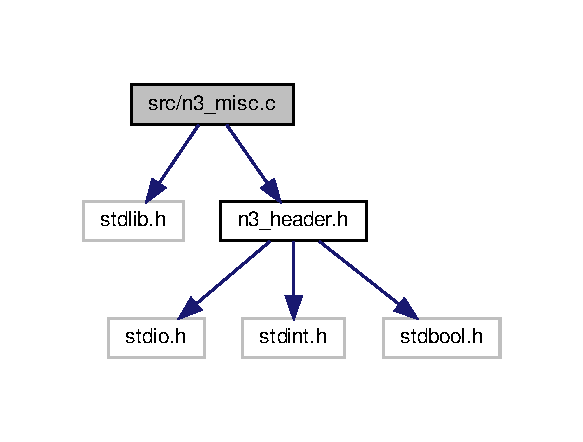
\includegraphics[width=280pt]{n3__misc_8c__incl}
\end{center}
\end{figure}
\subsection*{Functions}
\begin{DoxyCompactItemize}
\item 
double \hyperlink{n3__misc_8c_ad000cb3ea3bb9c116899973c4c382c64}{n3l\+\_\+misc\+\_\+rnd\+\_\+wp1} (void $\ast$data)
\begin{DoxyCompactList}\small\item\em Get random values between 0 and 1. \end{DoxyCompactList}\item 
double \hyperlink{n3__misc_8c_a20bef1a0eb58f93a1cd935ace0af28a8}{n3l\+\_\+misc\+\_\+rnd\+\_\+wn1} (void $\ast$data)
\begin{DoxyCompactList}\small\item\em Get random values between -\/1 and 0. \end{DoxyCompactList}\item 
double \hyperlink{n3__misc_8c_a31bb0c8231fc4206075182808c2b0348}{n3l\+\_\+misc\+\_\+rnd\+\_\+wpn1} (void $\ast$data)
\begin{DoxyCompactList}\small\item\em Get random values between -\/1 and 1. \end{DoxyCompactList}\item 
\hyperlink{structN3LArgs}{N3\+L\+Args} \hyperlink{n3__misc_8c_a22f4dc2ca9ee867a30c91565e37788d9}{n3l\+\_\+misc\+\_\+init\+\_\+arg} (void)
\begin{DoxyCompactList}\small\item\em Get the defaults arguments to build the network. \end{DoxyCompactList}\end{DoxyCompactItemize}


\subsection{Detailed Description}
This file contains functions to simplify working with the library. 

\begin{DoxyAuthor}{Author}
Davide Francesco Merico 
\end{DoxyAuthor}


\subsection{Function Documentation}
\mbox{\Hypertarget{n3__misc_8c_a22f4dc2ca9ee867a30c91565e37788d9}\label{n3__misc_8c_a22f4dc2ca9ee867a30c91565e37788d9}} 
\index{n3\+\_\+misc.\+c@{n3\+\_\+misc.\+c}!n3l\+\_\+misc\+\_\+init\+\_\+arg@{n3l\+\_\+misc\+\_\+init\+\_\+arg}}
\index{n3l\+\_\+misc\+\_\+init\+\_\+arg@{n3l\+\_\+misc\+\_\+init\+\_\+arg}!n3\+\_\+misc.\+c@{n3\+\_\+misc.\+c}}
\subsubsection{\texorpdfstring{n3l\+\_\+misc\+\_\+init\+\_\+arg()}{n3l\_misc\_init\_arg()}}
{\footnotesize\ttfamily \hyperlink{structN3LArgs}{N3\+L\+Args} n3l\+\_\+misc\+\_\+init\+\_\+arg (\begin{DoxyParamCaption}\item[{void}]{ }\end{DoxyParamCaption})}



Get the defaults arguments to build the network. 

Defaults values\+:
\begin{DoxyItemize}
\item bias\+: {\ttfamily 0.\+0} 
\item in\+\_\+size\+: {\ttfamily 1} 
\item h\+\_\+size\+: {\ttfamily N\+U\+LL} 
\item h\+\_\+layers\+: {\ttfamily 0} 
\item out\+\_\+size\+: {\ttfamily 1} 
\item act\+\_\+in\+: {\ttfamily N3\+L\+None} 
\item act\+\_\+h\+: {\ttfamily N\+U\+LL} 
\item act\+\_\+out\+: {\ttfamily N3\+L\+Sigmoid} 
\item rand\+\_\+arg\+: {\ttfamily N\+U\+LL} 
\item rand\+\_\+weight\+: {\ttfamily \&n3l\+\_\+misc\+\_\+rnd\+\_\+wp1} 
\end{DoxyItemize}

\begin{DoxyReturn}{Returns}
The defaults arguments listed above.
\end{DoxyReturn}
\begin{DoxySeeAlso}{See also}
\hyperlink{structN3LArgs}{N3\+L\+Args}, n3l\+\_\+network\+\_\+build, \hyperlink{n3__misc_8c_ad000cb3ea3bb9c116899973c4c382c64}{n3l\+\_\+misc\+\_\+rnd\+\_\+wp1} 
\end{DoxySeeAlso}
\mbox{\Hypertarget{n3__misc_8c_a20bef1a0eb58f93a1cd935ace0af28a8}\label{n3__misc_8c_a20bef1a0eb58f93a1cd935ace0af28a8}} 
\index{n3\+\_\+misc.\+c@{n3\+\_\+misc.\+c}!n3l\+\_\+misc\+\_\+rnd\+\_\+wn1@{n3l\+\_\+misc\+\_\+rnd\+\_\+wn1}}
\index{n3l\+\_\+misc\+\_\+rnd\+\_\+wn1@{n3l\+\_\+misc\+\_\+rnd\+\_\+wn1}!n3\+\_\+misc.\+c@{n3\+\_\+misc.\+c}}
\subsubsection{\texorpdfstring{n3l\+\_\+misc\+\_\+rnd\+\_\+wn1()}{n3l\_misc\_rnd\_wn1()}}
{\footnotesize\ttfamily double n3l\+\_\+misc\+\_\+rnd\+\_\+wn1 (\begin{DoxyParamCaption}\item[{void $\ast$}]{data }\end{DoxyParamCaption})}



Get random values between -\/1 and 0. 


\begin{DoxyParams}{Parameters}
{\em data} & Not used. Required by N3\+L\+Weight\+Generator. \\
\hline
\end{DoxyParams}
\begin{DoxyReturn}{Returns}
A random value between -\/1 and 0.
\end{DoxyReturn}
\begin{DoxySeeAlso}{See also}
n3l\+\_\+neuron\+\_\+build\+\_\+weights, \hyperlink{structN3LArgs}{N3\+L\+Args} 
\end{DoxySeeAlso}
\mbox{\Hypertarget{n3__misc_8c_ad000cb3ea3bb9c116899973c4c382c64}\label{n3__misc_8c_ad000cb3ea3bb9c116899973c4c382c64}} 
\index{n3\+\_\+misc.\+c@{n3\+\_\+misc.\+c}!n3l\+\_\+misc\+\_\+rnd\+\_\+wp1@{n3l\+\_\+misc\+\_\+rnd\+\_\+wp1}}
\index{n3l\+\_\+misc\+\_\+rnd\+\_\+wp1@{n3l\+\_\+misc\+\_\+rnd\+\_\+wp1}!n3\+\_\+misc.\+c@{n3\+\_\+misc.\+c}}
\subsubsection{\texorpdfstring{n3l\+\_\+misc\+\_\+rnd\+\_\+wp1()}{n3l\_misc\_rnd\_wp1()}}
{\footnotesize\ttfamily double n3l\+\_\+misc\+\_\+rnd\+\_\+wp1 (\begin{DoxyParamCaption}\item[{void $\ast$}]{data }\end{DoxyParamCaption})}



Get random values between 0 and 1. 


\begin{DoxyParams}{Parameters}
{\em data} & Not used. Required by N3\+L\+Weight\+Generator. \\
\hline
\end{DoxyParams}
\begin{DoxyReturn}{Returns}
A random value between 0 and 1.
\end{DoxyReturn}
\begin{DoxySeeAlso}{See also}
n3l\+\_\+neuron\+\_\+build\+\_\+weights, \hyperlink{structN3LArgs}{N3\+L\+Args} 
\end{DoxySeeAlso}
\mbox{\Hypertarget{n3__misc_8c_a31bb0c8231fc4206075182808c2b0348}\label{n3__misc_8c_a31bb0c8231fc4206075182808c2b0348}} 
\index{n3\+\_\+misc.\+c@{n3\+\_\+misc.\+c}!n3l\+\_\+misc\+\_\+rnd\+\_\+wpn1@{n3l\+\_\+misc\+\_\+rnd\+\_\+wpn1}}
\index{n3l\+\_\+misc\+\_\+rnd\+\_\+wpn1@{n3l\+\_\+misc\+\_\+rnd\+\_\+wpn1}!n3\+\_\+misc.\+c@{n3\+\_\+misc.\+c}}
\subsubsection{\texorpdfstring{n3l\+\_\+misc\+\_\+rnd\+\_\+wpn1()}{n3l\_misc\_rnd\_wpn1()}}
{\footnotesize\ttfamily double n3l\+\_\+misc\+\_\+rnd\+\_\+wpn1 (\begin{DoxyParamCaption}\item[{void $\ast$}]{data }\end{DoxyParamCaption})}



Get random values between -\/1 and 1. 


\begin{DoxyParams}{Parameters}
{\em data} & Not used. Required by N3\+L\+Weight\+Generator. \\
\hline
\end{DoxyParams}
\begin{DoxyReturn}{Returns}
A random value between -\/1 and 1.
\end{DoxyReturn}
\begin{DoxySeeAlso}{See also}
n3l\+\_\+neuron\+\_\+build\+\_\+weights, \hyperlink{structN3LArgs}{N3\+L\+Args} 
\end{DoxySeeAlso}

\hypertarget{n3__network_8c}{}\section{src/n3\+\_\+network.c File Reference}
\label{n3__network_8c}\index{src/n3\+\_\+network.\+c@{src/n3\+\_\+network.\+c}}


This file contains functions to work with \hyperlink{structN3LNetwork}{N3\+L\+Network} type.  


{\ttfamily \#include $<$stdlib.\+h$>$}\newline
{\ttfamily \#include $<$string.\+h$>$}\newline
{\ttfamily \#include \char`\"{}n3\+\_\+header.\+h\char`\"{}}\newline
{\ttfamily \#include \char`\"{}n3\+\_\+layer.\+h\char`\"{}}\newline
{\ttfamily \#include \char`\"{}n3\+\_\+neuron.\+h\char`\"{}}\newline
Include dependency graph for n3\+\_\+network.\+c\+:\nopagebreak
\begin{figure}[H]
\begin{center}
\leavevmode
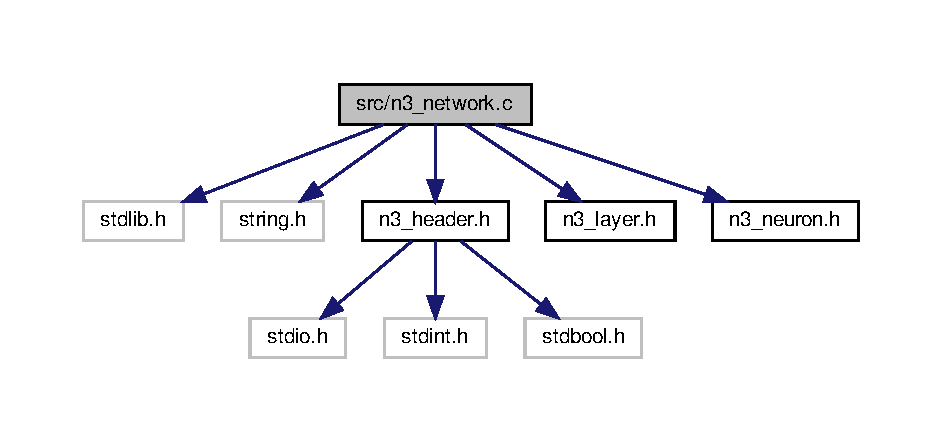
\includegraphics[width=350pt]{n3__network_8c__incl}
\end{center}
\end{figure}
\subsection*{Functions}
\begin{DoxyCompactItemize}
\item 
\hyperlink{structN3LNetwork}{N3\+L\+Network} $\ast$ \hyperlink{n3__network_8c_a5f87e1efebd658dd55d7d2ca1768bdba}{n3l\+\_\+network\+\_\+build} (\hyperlink{structN3LArgs}{N3\+L\+Args} args, double learn\+\_\+rate)
\begin{DoxyCompactList}\small\item\em Build a new network. \end{DoxyCompactList}\item 
void \hyperlink{n3__network_8c_a327ffd586b67f586743d72a146c4ea95}{n3l\+\_\+network\+\_\+free} (\hyperlink{structN3LNetwork}{N3\+L\+Network} $\ast$net)
\begin{DoxyCompactList}\small\item\em Free the network\textquotesingle{}s allocated memory. \end{DoxyCompactList}\end{DoxyCompactItemize}


\subsection{Detailed Description}
This file contains functions to work with \hyperlink{structN3LNetwork}{N3\+L\+Network} type. 

\begin{DoxyAuthor}{Author}
Davide Francesco Merico 
\end{DoxyAuthor}


\subsection{Function Documentation}
\mbox{\Hypertarget{n3__network_8c_a5f87e1efebd658dd55d7d2ca1768bdba}\label{n3__network_8c_a5f87e1efebd658dd55d7d2ca1768bdba}} 
\index{n3\+\_\+network.\+c@{n3\+\_\+network.\+c}!n3l\+\_\+network\+\_\+build@{n3l\+\_\+network\+\_\+build}}
\index{n3l\+\_\+network\+\_\+build@{n3l\+\_\+network\+\_\+build}!n3\+\_\+network.\+c@{n3\+\_\+network.\+c}}
\subsubsection{\texorpdfstring{n3l\+\_\+network\+\_\+build()}{n3l\_network\_build()}}
{\footnotesize\ttfamily \hyperlink{structN3LNetwork}{N3\+L\+Network}$\ast$ n3l\+\_\+network\+\_\+build (\begin{DoxyParamCaption}\item[{\hyperlink{structN3LArgs}{N3\+L\+Args}}]{args,  }\item[{double}]{learn\+\_\+rate }\end{DoxyParamCaption})}



Build a new network. 

\begin{DoxyNote}{Note}
Layers are built in order\+: Input, Hidden, Output. 

Bias neurons, if specified, are added as last neuron in neurons list.
\end{DoxyNote}

\begin{DoxyParams}{Parameters}
{\em args} & Parameters to initialize the network. \\
\hline
{\em learn\+\_\+rate} & Initial learning rate when used backpropagation. \\
\hline
\end{DoxyParams}
\begin{DoxyReturn}{Returns}
The new network if built successfully, otherwise N\+U\+LL.
\end{DoxyReturn}
\begin{DoxySeeAlso}{See also}
\hyperlink{structN3LArgs}{N3\+L\+Args}, \hyperlink{n3__misc_8c_a22f4dc2ca9ee867a30c91565e37788d9}{n3l\+\_\+misc\+\_\+init\+\_\+arg}, \hyperlink{structN3LNetwork}{N3\+L\+Network}, \hyperlink{n3__network_8c_a327ffd586b67f586743d72a146c4ea95}{n3l\+\_\+network\+\_\+free}, \hyperlink{n3__file_8c_a4fef76548ed87845dceafaa9527a83d0}{n3l\+\_\+file\+\_\+import\+\_\+network} 
\end{DoxySeeAlso}
\mbox{\Hypertarget{n3__network_8c_a327ffd586b67f586743d72a146c4ea95}\label{n3__network_8c_a327ffd586b67f586743d72a146c4ea95}} 
\index{n3\+\_\+network.\+c@{n3\+\_\+network.\+c}!n3l\+\_\+network\+\_\+free@{n3l\+\_\+network\+\_\+free}}
\index{n3l\+\_\+network\+\_\+free@{n3l\+\_\+network\+\_\+free}!n3\+\_\+network.\+c@{n3\+\_\+network.\+c}}
\subsubsection{\texorpdfstring{n3l\+\_\+network\+\_\+free()}{n3l\_network\_free()}}
{\footnotesize\ttfamily void n3l\+\_\+network\+\_\+free (\begin{DoxyParamCaption}\item[{\hyperlink{structN3LNetwork}{N3\+L\+Network} $\ast$}]{net }\end{DoxyParamCaption})}



Free the network\textquotesingle{}s allocated memory. 

\begin{DoxyNote}{Note}
It also free all network\textquotesingle{}s layers and neurons.
\end{DoxyNote}
\begin{DoxySeeAlso}{See also}
\hyperlink{n3__layer_8c_ad58e1630c1b7fc5da03d54cf63c394d9}{n3l\+\_\+layer\+\_\+free}, \hyperlink{n3__neuron_8c_a3f9b33cd97e88140c8adadb483b1cea5}{n3l\+\_\+neuron\+\_\+free}, \hyperlink{n3__network_8c_a5f87e1efebd658dd55d7d2ca1768bdba}{n3l\+\_\+network\+\_\+build} 
\end{DoxySeeAlso}

%--- End generated contents ---

% Index
\backmatter
\newpage
\phantomsection
\clearemptydoublepage
\addcontentsline{toc}{chapter}{Index}
\printindex

\end{document}
